\chapter{Apêndice A - Teste Baseado em Modelo para Linha de Produto de Software: Uma Revisão Sistemática da Literatura}
\label{sec:apendice}


\subsection{Processo de Pesquisa}
O processo de pesquisa foi elaborado seguindo padrões de processos \cite{kitchenham2004procedures}, \cite{nakagawa2017revisao}, \cite{keele2007guidelines} em que tais processos envolvem 3 fases: Planejamento, Condução e Documentação dos resultados.

De forma resumida a fase de planejamento tem como objetivo identificar a real necessidade, motivação para a execução da RSL, porém antes de se iniciar uma RSL é fundamental identificar se já não existe um estudo secundário referente ao tema proposto.

Embora isso seja uma premissa, para este trabalho adotamos uma pesquisa prévia para identificar trabalhos secundários referente ao tema. Foi encontrado um estudo secundário desenvolvido por \cite{isa2017model}, porém este trabalho não seguiu muitos dos padrões recomendados por \cite{kitchenham2004procedures}. Ele apresenta dados superficiais interessantes porém com inúmeras ameaças à validade dos resultados e sem condição alguma de ser replicado.

Posterior a fase de planejamento, a condução é a busca e a seleção dos trabalhos relacionados ao tema. Nesta RSL realizamos a busca automática nas bases digitais e após a busca manual, em seguida, adotamos a utilização do \textit{Snowballing} (\citealp{wohlin2014guidelines}) que consiste em uma busca manual ou automática utilizando a lista de referências de trabalhos relevantes. A execução desta técnica consiste de duas etapas, o reverso que faz a avaliação da lista de referências de um estudo relevante e o avante que que consiste em analisar a lista de citações.

Para este trabalho adotamos o \textit{Snowballing} reverso por causa da quantidade de trabalhos selecionados. Já na última fase que é a de documentação, descrevem-se os resultados afim de se compartilhar e permitir a replicação do estudo por outros pesquisadores. Na \ref{fig:processo} apresenta o processo de RSL adotado neste estudo.

\newpage
\begin{figure}[htb]
	\centering
	\caption{Visão do processo de RSL, adaptado de \cite{nakagawa2017revisao}}
	\includegraphics[scale=.57]{processo.png}
	\label{fig:processo}
\end{figure}

De forma resumida os procedimentos do processo de pesquisa \ref{fig:processo} foram estabelecidos da seguinte forma:

\begin{itemize}
	\item Definição das questões de pesquisa;
	
	\item Realizar o planejamento da pesquisa;
	
	\item Selecionar as bases de dados eletrônicas e os mecanismos de busca indexada;
	
	\item definir as palavras chaves para compor a \textit{string} de busca principal para obtenção dos estudos primários e secundários.
	
	\item Compor as palavras chaves e variações utilizando "AND"e "OR" para obtenção
	dos estudos primários;
	
	\item Selecionar os estudos relevantes se baseando nos critérios de inclusão e exclusão;
	
	\item Realizar a classificação dos trabalhos conforme grau de importância e relevância a pesquisa;
	
	\item Extrair informações; e
	
	\item Realizar discussões a respeito dos estudos dados extraídos dos estudos selecionados.
	
\end{itemize}

\subsection{Questões de Pesquisa}
O objetivo desta RSL é obter um entendimento sobre a forma como teste baseado em modelo (TBM) é aplicado em uma linha de produto de software (LPS). E quando aplicado, se possui apoio ao gerenciamento de variabilidade.
A formulação da questão de pesquisa, baseada no objetivo principal  apresenta-se a seguir:

\textbf{- QP01:} Em quais domínios TBM tem sido aplicado em LPS?

\textbf{- QP02:} Quais abordagens têm sido utilizadas no TBM de LPS?

\textbf{- QP03:} Qual o tipo de problema em LPS que TBM tem solucionado?

\textbf{- QP04:} Como variabilidade é tratada no TBM de LPS?

\textbf{- QP05:} Como TBM apoia o teste de requisitos não-funcionais?

\textbf{- QP06:} A geração de casos de testes utiliza-se de artefatos ou ferramentas?

\textbf{- QP07:} Quais artefatos de LPS têm sido considerados no TBM?

\textbf{- QP08:} \textit{Binding time} afeta a aplicação de TBM em LPS?

\textbf{- QP09:} Como as técnicas e as atividades de TBM para LPS têm sido avaliadas?

\textbf{- QP10:} É realizado a rastreabilidade em TBM para LPS?

\textbf{- QP11:} Quais as soluções propostas para TBM?

\subsection{Estratégia de Busca para Seleção de Estudos}
A estratégia de busca de uma RSL segundo \cite{keele2007guidelines} é encontrar os estudos primários relevantes à pesquisa, baseado na definição das palavras chaves e locais onde serão realizadas as buscas, seja manual ou automatizada. O processo de busca deve ser amplo para atingir uma quantidade elevada de estudos.

Como estratégia de busca de estudos primários foi definido que a busca seria de acordo com as fontes de pesquisa, o idioma dos trabalhos, os tipos dos estudos, as palavras chaves e, respectivamente, a \textit{string} de busca, conforme segue:

\begin{itemize}
	\item Fontes de pesquisa: bases de dados eletrônicas indexadas (IEEE, ACM, ScienceDirect, Scopus, IET Digtial Library, Google \textit{Scholar}, Springer);
	
	\item Idioma dos trabalhos: inglês;
	
	\item Tipo de publicação: estudos primários publicados em periódicos, conferências
	e capítulos de livros por terem sido avaliados por seus pares;
	
	\item Palavras-chave: \textit{Software, product line, product-line, product family, product-family, product-families, family of products, variability, model-based testing, model based testing}, MBT;
	
	\item Strings de busca e sequências de consulta: combinação das palavras-chave e suas variações utilizando os operadores lógicos \textit{AND} e \textit{OR}, conforme apresentado na \ref{fig:string}:
\end{itemize}

\begin{figure}[htb]
	\centering
	\caption{\textit{String} de Busca geral}
	\includegraphics[scale=.35]{string.png}
	\label{fig:string}
\end{figure}

\subsubsection{Fontes de Busca}
As bibliotecas digitais utilizadas para a coleta automática neste estudo são apresentadas na \ref{table:fontes}

\begin{table}[]
	\centering
	\caption{Máquinas de busca utilizadas}
	\label{table:fontes}
	\begin{tabular}{|l|l|}
		\hline
		\textbf{Fonte Automática} & \textbf{Endereço eletrônico}                               \\ \hline
		ACM Digital Library  & http://dl.acm.org/                                         \\ \hline
		IEEE Xplore          & http://ieeexplore.ieee.org/                                \\ \hline
		ScienceDirect        & http://www.sciencedirect.com/                              \\ \hline
		Scopus               & http://www.info.sciverse.com/scopus/                       \\ \hline
		Springer             & http://www.springer.com/                                   \\ \hline
		Google Scholar      & https://scholar.google.com                                 \\ \hline
		IET  Digital Library & http://digital-library.theiet.org/content/journals/iet-sen \\ \hline
	\end{tabular}
\end{table}

Além da pesquisa nas bases de dados eletrônicas indexadas relacionadas na \ref{table:fontes} na busca manual foi realizado a consulta em sites de periódicos e conferências. Foram considerados estudos de conferências citadas na \ref{table:manual} e os periódicos da \ref{table:jornal} nos últimos dez anos e, por estarem correlacionados a área.

\begin{table}[]
	\centering
	\caption{Lista de conferências para busca manual}
	\label{table:manual}
	\begin{tabular}{|l|l|}
		\hline
		\textbf{Sigla} & \textbf{Conferência}                                           \\ \hline
		ICECCS         & Engineering of Complex Computer Systems                        \\ \hline
		AISE           & Advanced Information Systems Engineering                       \\ \hline
		ICST           & International Conference on Software Testing                   \\ \hline
		ICIS           & Computer and Information Science                               \\ \hline
		ACM SIGSOFT    & Software Engineering Notes                                     \\ \hline
		MSIS           & Workshop on Variability Modeling of Software-Intensive Systems \\ \hline
		ISPL           & International Software Product Line Conference                 \\ \hline
		ICSTSS         & International Conference on Testing Software and Systems       \\ \hline
		QA\&TEST       & International Conference on Software QA and Testing            \\ \hline
		IFIP           & International Conference on Testing Software and Systems       \\ \hline
	\end{tabular}
\end{table}

\begin{table}[]
	\centering
	\caption{Lista de periódicos para busca manual}
	\label{table:jornal}
	\begin{tabular}{|l|l|}
		\hline
		\textbf{Sigla} & \textbf{Journal}                    \\ \hline
		ESE            & Empirical Software Engineering      \\ \hline
		JSS            & Journal of Systems and Software     \\ \hline
		IST            & Information and Software Technology \\ \hline
		ASC            & Applied Soft Computing              \\ \hline
		SQJ            & Software Quality Journal            \\ \hline
		SCP            & Science of Computer Programming     \\ \hline
	\end{tabular}
\end{table}

\newpage
\subsection{Estratégia de Seleção}

\subsubsection{Processo de Seleção}
O processo de seleção dos estudos foi realizado em seis etapas conforme a \ref{fig:selecao}, descritos a seguir:
\begin{figure}[htb]
	\centering
	\caption{Processo de condução de seleção da RSL}
	\includegraphics[scale=.55]{fluxo.png}
	\label{fig:selecao}
\end{figure}

\begin{itemize}
	\item \textbf{Utilizar \textit{String} de busca nas bases:} a utilização da \textit{string} geral foi adaptada a cada um das bibliotecas digitais utilizadas, pois existe uma variação de sintaxe para cada uma delas. Concluída a busca inicial, foi realizada a leitura do título, resumo e aplicados os critérios de inclusão e exclusão;
	
	\item \textbf{Realizar a busca Manual:} Foi feito o acesso aos periódicos e realizado a busca. Concluído a busca, foi realizada a leitura do título, resumo e aplicados os critérios de inclusão e exclusão. Após, realizou-se a ordenação conforme a avaliação de qualidade. 
	
	\item \textbf{Unificação das duas listas:} após as buscas automáticas e manuais, os resultados da 1° Lista e da 2° Lista foram unificados gerando uma 3° Lista que foi utilizada em uma pré-seleção final dos estudos primários.
	
	\item \textbf{Seleção Final dos estudos primários:} nessa etapa, foi realizada a leitura da introdução e conclusão dos trabalhos selecionados, para se gerar uma 4° lista. Nesta etapa, trabalhos que geraram incerteza ou dúvida foram lidos.
	
	\item \textbf{Realização do \textit{snowballing}:} o \textit{snowballing} consiste na busca de novos estudos primários baseada na lista de referência dos estudos selecionados na fase final. Neste trabalho adotamos o tipo reverso de \textit{snowballing} buscando por estudos prévios.
	
	\item \textbf{Seleção final pós \textit{snowballing}:} com a lista de estudos, após o \textit{snowballing} procedeu-sea leitura completa e extração de dados de tais estudos.
\end{itemize}

Com o objetivo de selecionar os estudos mais relevantes e contribuir para responder as questões da pesquisa para este estudo secundário, foram definidos os critérios de inclusão e exclusão apresentados a seguir.

\subsubsection{Critérios de Inclusão:} Foram incluídos os trabalhos:

\begin{itemize}
	\item que abordam técnicas de TBM em LPS;
	\item publicações a partir dos últimos dez anos, afim de evitar versões mais antigas de trabalhos recentes;
	\item abordam variabilidade em LPS.
\end{itemize}


\subsubsection{Critérios de Exclusão:} Foram excluídos os trabalhos:

\begin{itemize}
	\item que não abordam técnicas de TBM em LPS;
	\item em que o texto do estudo não está completo;
	\item em outro que não seja inglês;
	\item que são chamadas de workshops, palestras e seminários;
	\item com número de páginas abaixo de 4;
	\item duplicados;
	\item recuperados por meio eletrônico em formatos que não forrem PDF (Portable Document Format), DOC/DOCX (Processador de Texto MicrosoftWord) ou ODT (Processador de Texto do Open Office);
	\item indisponíveis, que não puderam ser recuperados;
\end{itemize}

\subsection{Avaliação de Qualidade dos Estudos}

Para a avaliação da qualidade dos trabalhos foi aplicado questionário com três perguntas após a leitura dos mesmos:

\begin{itemize}
	\item O estudo é revisado aos pares?
	\item O objetivo do estudo está claro?
	\item A proposta de estudo foi avaliada/validada?
\end{itemize}

Para cada pergunta houve três alternativas, em que só uma delas podia ser escolhida;

Trabalhos com a alternativa "Não" como resposta, foram descartados automaticamente. Estudos que tiverem a alternativa "Parcialmente", foi feita uma nova leitura para não deixar dúvida do nível de contribuição.

\subsection{Estratégia de Extração de Dados}
\label{sec:estrategia}
A extração de dados foi projetada para coletar a informação necessária para responder as questões de pesquisa, assim como analisar os estudos dos critérios de seleção. 

Para isso, foi criada \ref{table:criterios} com critérios de qualidade e uma lista de atributos.

\begin{table}[]
	\centering
	\caption{Critérios de qualidade aplicado aos trabalhos resultantes}
	\label{table:criterios}
	\begin{tabular}{|l|l|l|}
		\hline
		\multirow{2}{*}{\textbf{Critério de qualidade dos trabalhos}}                     & \multicolumn{2}{l|}{\textbf{Classificação}} \\ \cline{2-3} 
		& \textbf{Sim (1)}     & \textbf{Não (0)}     \\ \hline
		O trabalho descreve claramente o objetivo da pesquisa?              &                      &                      \\ \hline
		O domínio de atuação está condizente com a área de pesquisa?        &                      &                      \\ \hline
		O estudo passou por algum processo de avaliação?                    &                      &                      \\ \hline
		Houve uma coleta de dados apropriada?                               &                      &                      \\ \hline
		Houve uma análise apropriada dos dados?                             &                      &                      \\ \hline
		O trabalho apresenta resultados condizentes com seus objetivos?     &                      &                      \\ \hline
		O resultado contribui para o processo realizado para esta pesquisa? &                      &                      \\ \hline
	\end{tabular}
\end{table}


Tal lista de atributos foi elaborada para ser extraída dos estudos selecionados, conforme apresentada a seguir:

\begin{itemize}
	\item Título;
	\item Autor(es);
	\item Ano de publicação;
	\item Fonte da publicação;
	\item Tipo da publicação;
	\item Tipo do documento;
	\item Domínio aplicado;
	\item Inclui ou não variabilidade;
	\item Se aborda \textit{feature interaction};
	\item Método de execução;
	\item Técnica de teste utilizada;
	\item Nível de teste aplicado;
	\item Abordagem de teste utilizada;
	\item Qual o nível de cobertura;
	\item Rastreabilidade;
	\item Propósito do TBM;
	\item Se apoia o teste de requisito não funcional;
	\item Artefato de origem;
	\item Artefato intermediário;
	\item Utilização de ferramentas;
	\item \textit{Binding Time};
	\item Se atividades de TBM são avaliadas;
	\item Resultados da pesquisa;
	\item Método de coleta das evidências;
	\item Local da validação;
	\item Tipo de contribuição.
	
\end{itemize}


\subsection{Validação do Planejamento da RSL}

Nesta avaliação de protocolo foi utilizada a escala Likert para coletar a opinião dos pesquisadores, por facilitar a construção da pesquisa, coleta e análise de dados \cite{li2013novel}.
O questionário tem as seguintes respostas como opção aos pesquisadores participantes:
\begin{itemize}
	\item Discordo totalmente (Peso 1): quando o protocolo não atende de nenhuma forma os critérios da questão;
	\item Discordo parcialmente (Peso 2): quando o protocolo não atende os critérios da	questão;
	\item Neutro (Peso 3): quando o protocolo não deixa claro se atende ou não os critérios da questão;
	\item Concordo parcialmente (Peso 4): quando o protocolo atende parcialmente os critérios da questão;
	\item Concordo totalmente (Peso 5): quando o protocolo atende totalmente os critérios da questão;
\end{itemize}

Ao final foi disponibilizada uma opção para a sugestão de melhorias referentes ao protocolo. O objetivo principal dessa avaliação foi refinar o protocolo com base nas respostas e sugestões dos especialistas.


\subsection{Avaliação do Protocolo da RSL}

O questionário de avaliação do protocolo\footnote[1]{Disponível em: https://goo.gl/forms/BfezYRLoojUOjBRv2 - Acessado em 16/06/2017} foi enviado para 7 pesquisadores da área de Sistemas de Informação, assim, foram obtidas 5 respostas. 

\begin{table}[]
	\centering
	\caption{Pesquisadores que avaliaram o protocolo da RSL}
	\label{table:avaliadores}
	\begin{tabular}{|l|l|l|}
		\hline
		\multicolumn{1}{|c|}{\textbf{\begin{tabular}[c]{@{}c@{}}Nível de \\ Títulação\end{tabular}}} & \multicolumn{1}{c|}{\textbf{Instituição}} & \multicolumn{1}{c|}{\textbf{Área de Pesquisa}} \\ \hline
		Doutor & Universidade Tecnologica Federal do Parana & Sistemas de Informação \\ \hline
		Doutor & Universidade Federal do Pampa & Engenharia de Software \\ \hline
		Doutor & Universitat Politècnica de València Espanha & Engenharia Elétrica \\ \hline
		Doutor & Universidade Federal do Paraná & Engenharia de Software \\ \hline
		Mestre & Instituo SENAI de Tecnologia em Metalmecânica & Engenharia Elétrica \\ \hline
	\end{tabular}
\end{table}

Os especialistas convidados realizaram uma avaliação muito produtiva, todos consideram que pode ser encontrada alguma questão importante sobre TBM em LPS com foco em variabilidade. A grande maioria também concorda que a String de busca está adequada com base nas perguntas de pesquisa.

Outro ponto em que concordam que as fontes e os tipos de busca cobrem os estudos relevantes, porém com relação aos critérios de inclusão e exclusão, alguns discordaram como, por exemplo, a seleção de trabalhos se limitar a somente os últimos 10 anos de pesquisas.

Houve um questionamento sobre a análise de qualidade dos trabalhos, neste caso foi sugerido a aplicação do questionário de critério de qualidade da \ref{table:criterios}

Uma sugestão foi utilizar a avaliação pelo número de citações, essa sugestão foi aplicada em conjunto com o questionário de critérios onde surgiu a tabela \ref{table:top10} com os 10 trabalhos com maior relevância sobre o tema proposto.

\newpage
\section{Execução da RSL}
Nesta seção são apresentados os passos executados a partir do planejamento da RSL.
\subsection{Busca Eletrônica}
As buscas para esta RSL foram executadas no período de Julho de 2017 à Setembro de 2017. A busca envolveu duas fases: a busca automática de estudos por meio dos mecanismos de dados eletrônicos e a busca manual em conferências e periódicos.

A partir da \textit{string} geral apresentada na \ref{fig:string}, cada base eletrônica teve sua derivação de adaptação.

As \textit{strings} utilizadas foram:

\begin{itemize}
	\item ACM Digital Library:
	
	(	\textit{"software" +"product line ''"product-lin''"product family''"product-family''\\	
		"product-families''	"family of products''"variability" +"model-based testing''\\"model based testing''"MBT"})
	
	\item Google Academic:
	
	(\textit{"Software") AND ("product line" or "product-line" or "product family" or \\"product-family" or "product-families" or "family of products" or "variability") AND ("model-based testing" or "model based testing" or "MBT"})
	
	\item IEEE:
	
	(\textit{("software") AND ("product line" OR "product-line" OR "product family" OR \\"product-family" OR "product-families" OR "family of products" OR "variability") AND ("model-based testing" OR "model based testing" OR "MBT")})
	
	\item Springer:
	
	(\textit{(software)  AND  (''product line'' or ''product-line'' or ''product family'' or \\''product-family'' or ''product-families'' or ''family of products'' or ''variability'')  AND  (''model-based testing'' or ''model based testing'' or MBT)}
	
	\item Scopus:
	
	\textit{( TITLE-ABS-KEY ( software )  AND  TITLE-ABS-KEY ( {product line}  OR  \\{product-line}  OR  {product family}  OR  {product-family}  OR  {product-families}  OR  {family of products}  OR  {variability} )  AND  TITLE-ABS-KEY ( {model-based testing}  OR  {model based testing}  OR  {MBT} ) )  AND  ( PUBYEAR  $>$  2005 ) }
	
	\item Science Direct:
	
	\textit{("software") AND ("product line" OR "product-line" OR "product family" OR \\"product-family" OR "product-families" OR "family of products" OR "variability") AND ("model-based testing" OR "model based testing" OR "MBT")}
	
	\item IET digital library:
	
	\textit{(("software") AND ("product line" OR "product-line" OR "product family" OR \\"product-family" OR "product-families" OR "family of products" OR "variability") AND ("model-based testing" OR "model based testing" OR "MBT"))}
\end{itemize}

Esse procedimento totalizou em 266 estudos recuperados em um primeiro momento, isso porque alguns trabalhos se repetem em dois ou mais motores de busca, ainda assim Science Direct retornou a maior parte como visto na \ref{table:buscaauto}.

Durante o processo de busca os trabalhos retornados foram sendo classificados conforme os critérios de inclusão e exclusão. Ao final desta etapa, 40 estudos foram aceitos e compuseram a 1° Lista, assim considerado para análise futura. 179 artigos foram rejeitados por não atenderem os critérios de inclusão e 23 foram classificados como duplicados por cada biblioteca digital num total de 47 repetições alternadas entre os trabalhos nos motores de busca.

\begin{figure}[htb]
	\centering
	\includegraphics[scale=0.60]{selecao.png}
	\caption{Resultado de classificação da busca automática}
	\label{fig:grafico}
\end{figure}


\begin{table}[]
	\centering
	\caption{Trabalhos retornados e aceitos das fontes eletrônicas}
	\label{table:buscaauto}
	\resizebox{\textwidth}{!}{%
		\begin{tabular}{|l|c|c|c|c|}
			\hline
			\multicolumn{1}{|c|}{\textbf{Fonte Eletrônica}} & \textbf{Artigos Retornados} & \textbf{Artigos Aceitos} & \textbf{Duplicados} & \textbf{Rejeitados} \\ \hline
			Springer & 7 & 5 & 1 & 1 \\ \hline
			Scopus & 62 & 10 & 21 & 31 \\ \hline
			Science Direct & 125 & 7 & 0 & 118 \\ \hline
			Empirical Software Engineering & 15 & 0 & 0 & 15 \\ \hline
			IEEE Software & 25 & 0 & 0 & 25 \\ \hline
			IET Digital Library & 9 & 0 & 0 & 9 \\ \hline
			Google Academic & 3 & 2 & 0 & 1 \\ \hline
			ACM & 20 & 16 & 1 & 3 \\ \hline
			\multicolumn{1}{|c|}{Total} & \textbf{266} & \textbf{40} & \textbf{23} & \textbf{203} \\ \hline
		\end{tabular}%
	}
\end{table}

Já a \ref{fig:paticipacao} apresenta a participação de cada base no montante de trabalhos selecionados. No gráfico não é apresentada a base IET Digital Library, devido a classificação inicial não ter artigos aceitos. Embora alguns estudos da busca manual sejam da biblioteca acima citada, porém, sendo classificados como duplicados.

\begin{figure}[htb]
	\centering
	\includegraphics[scale=0.60]{participacao.png}
	\caption{Classificação por motor de busca}
	\label{fig:paticipacao}
\end{figure}
\newpage
\subsection{Busca Manual}
Na execução da busca manual, trabalhos com pouca relevância foram descartados permanentemente. Durante esta etapa foram lidos primeiramente o título e as palavra-chave dos artigos para incluí-los. 

Para os trabalho com um título abrangente, o \textit{abstract} também foi lido com o intuito de observar se o trabalho realmente era candidato a responder as questões de pesquisa. Ao final desta etapa foram retornados 21 trabalhos provenientes de conferências e periódicos sendo 12 foram selecionados para a etapa final. Os demais trabalhos foram rejeitados ou vieram duplicados semelhante a de alguma busca automática realizada.

\begin{table}[]
	\centering
	\caption{Fontes das buscas manuais com trabalhos retornados e aceitos.}
	\label{table:manualtabela}
	\resizebox{\textwidth}{!}{%
		\begin{tabular}{|l|c|c|c|}
			\hline
			\textbf{Fonte} & \textbf{\begin{tabular}[c]{@{}c@{}}Artigos\\ Retornados\end{tabular}} & \textbf{\begin{tabular}[c]{@{}c@{}}Artigos\\ Aceitos\end{tabular}} & \textbf{\begin{tabular}[c]{@{}c@{}}Artigos\\ Rejeitados\end{tabular}} \\ \hline
			Software \& Systems Modeling & 1 & 1 & 0 \\ \hline
			Model Driven Engineering Languages and Systems & 1 & 0 & 1 \\ \hline
			PESC-COPPE/UFRJ & 1 & 0 & 1 \\ \hline
			Engineering of Complex Computer Systems (ICECCS) & 1 & 1 & 0 \\ \hline
			Software Quality Journal & 1 & 1 & 0 \\ \hline
			Software Testing, Verification and Validation (ICST) & 1 & 1 & 0 \\ \hline
			Computer and Information Science (ICIS) & 1 & 1 & 0 \\ \hline
			ACM SIGSOFT Software Engineering Notes & 1 & 1 & 0 \\ \hline
			\begin{tabular}[c]{@{}l@{}}Workshop on Variability Modeling \\ of Software-Intensive Systems\end{tabular} & 1 & 0 & 1 \\ \hline
			International Software Product Line Conference & 1 & 0 & 1 \\ \hline
			IEEE software & 1 & 0 & 1 \\ \hline
			Periódico não especificado & 8 & 4 & 4 \\ \hline
			Conferências não especificadas & 2 & 2 & 0 \\ \hline
			\multicolumn{1}{|c|}{\textbf{Total}} & \textbf{21} & \textbf{12} & \textbf{9} \\ \hline
		\end{tabular}%
	}
\end{table}


Vale ressaltar que algumas fontes que não foram previstas inicialmente \ref{table:manual} retornaram trabalhos, porém muitos deles não foram aceitos \ref{table:manualtabela}.


\subsection{União das listas Automática e Manual}
Após a realização da busca manual, foi realizada uma união da lista 1 com a lista 2, busca automática com a manual. Surgiu então a lista 3, onde foi realizada a primeira seleção antes do \textit{snowballing}

\textit{\subsection{Snowballing}}
Nesta etapa, para direcionar o foco somente ao tema optamos por realizar o \textit{snowballing} reverso, onde avaliamos as referências dos estudos da 3° lista e buscamos encontrar trabalhos que pudessem contribuir para a RSL. Na realização do \textit{snowballing} foram retornados 10 estudos relacionados diretamente ao tema (\ref{table:snow}), que possam ser aplicados os critérios de seleção e qualidade. 


\begin{table}[]
	\centering
	\caption{Estudos retornados do \textit{snowballing} reverso}
	\label{table:snow}
	\resizebox{\textwidth}{!}{%
		\begin{tabular}{|c|l|c|l|c|}
			\hline
			\textbf{ID} & \multicolumn{1}{c|}{\textbf{Artigo de Origem}}                                                                                                              & \textbf{ID} & \multicolumn{1}{c|}{\textbf{Artigo Retornado}}                                                                                                   & \textbf{Status}                                                \\ \hline
			T5          & MPLM MaTeLo Product Line Manager                                                                                                                          & N/A         & \begin{tabular}[c]{@{}l@{}}An approach to derive usage models\\ variants for model-based\end{tabular}                                            & \begin{tabular}[c]{@{}c@{}}Duplicado/\\ Rejeitado\end{tabular} \\ \hline
			T8          & \begin{tabular}[c]{@{}l@{}}Deriving Usage Model Variants for Model-based Testing:\\  An Industrial Case Study\end{tabular}                                  & T37         & \begin{tabular}[c]{@{}l@{}}Relating Variability Modeling and Model-Based \\ Testing for Software Product Lines Testing\end{tabular}              & Aceito                                                         \\ \hline
			T10         & \begin{tabular}[c]{@{}l@{}}Model-Based Test Design of Product Lines: \\ Raising Test Design to the Product Line Level\end{tabular}                          & T38         & \begin{tabular}[c]{@{}l@{}}An Evaluation of Model-Based Testing\\  in Embedded Applications\end{tabular}                                         & Aceito                                                         \\ \hline
			T10         & \begin{tabular}[c]{@{}l@{}}Model-Based Test Design of Product Lines: \\ Raising Test Design to the Product Line Level\end{tabular}                          & T39         & \begin{tabular}[c]{@{}l@{}}Assessing Software Product Line Testing \\ Via Model-Based Mutation An Application to Similarity Testing\end{tabular} & Aceito                                                         \\ \hline
			T24         & \begin{tabular}[c]{@{}l@{}}A Model Based Testing Approach \\ for Model-Driven Development and Software Product Lines\end{tabular}                           & T36         & \begin{tabular}[c]{@{}l@{}}Automated model-based testing using the \\ UML testing profile and QVT\end{tabular}                                   & Aceito                                                         \\ \hline
			T20         & \begin{tabular}[c]{@{}l@{}}PLETS - A PRODUCT LINE \\ OF MODEL-BASED TESTING TOOLS\end{tabular}                                                              & T41         & \begin{tabular}[c]{@{}l@{}}Model-based Testing of System Requirements \\ using UML Use Case Models\end{tabular}                                  & Aceito                                                         \\ \hline
			T9          & \begin{tabular}[c]{@{}l@{}}Model-based Software Product Line Testing by Coupling \\ Feature Models with Hierarchical Markov Chain Usage Models\end{tabular} & T42         & \begin{tabular}[c]{@{}l@{}}Successive refinement of models for model-based testing\\  to increase system test effectiveness\end{tabular}         & Aceito                                                         \\ \hline
			T20         & \begin{tabular}[c]{@{}l@{}}PLETS - A PRODUCT LINE \\ OF MODEL-BASED TESTING TOOLS\end{tabular}                                                              & T43         & A Software Product Line for Model-Based Testing Tools                                                                                            & Aceito                                                         \\ \hline
			T21         & \begin{tabular}[c]{@{}l@{}}Top-Down and Bottom-Up Approach \\ for Model-Based Testing of Product Lines\end{tabular}                                         & T44         & \begin{tabular}[c]{@{}l@{}}Reusing State Machines for Automatic Test \\ Generation in Product Lines\end{tabular}                                 & Aceito                                                         \\ \hline
			T5          & MPLM MaTeLo Product Line Manager                                                                                                                          & T40         & \begin{tabular}[c]{@{}l@{}}Automated and Scalable T-wise Test Case \\ Generation Strategies for Software Product Lines\end{tabular}              & Aceito                                                         \\ \hline
		\end{tabular}%
	}
\end{table}


\subsection{Seleção Final}

Ao final do \textit{snowballing} foi realizada a somatória da busca digital mais a manual e o \textit{snowballing} totalizando 61 trabalhos que continham potencial para a seleção final. Assim, foi realizada a última seleção, restando apenas 44 estudos para a lista de extração de dados. 17 trabalhos foram descartados por não terem critérios bem definidos. 

Nessa etapa a seleção foi mais enfática com relação ao tema, buscando nivelar os critérios e leitura do conteúdo.
Na \ref{fig:qtdano} é possível visualizar um interesse crescente pelo tema, o que motiva um maior estudo sobre o tema.


\begin{figure}[htb]
	\centering
	\caption{Distribuição dos trabalhos selecionados nos últimos 10 anos}
	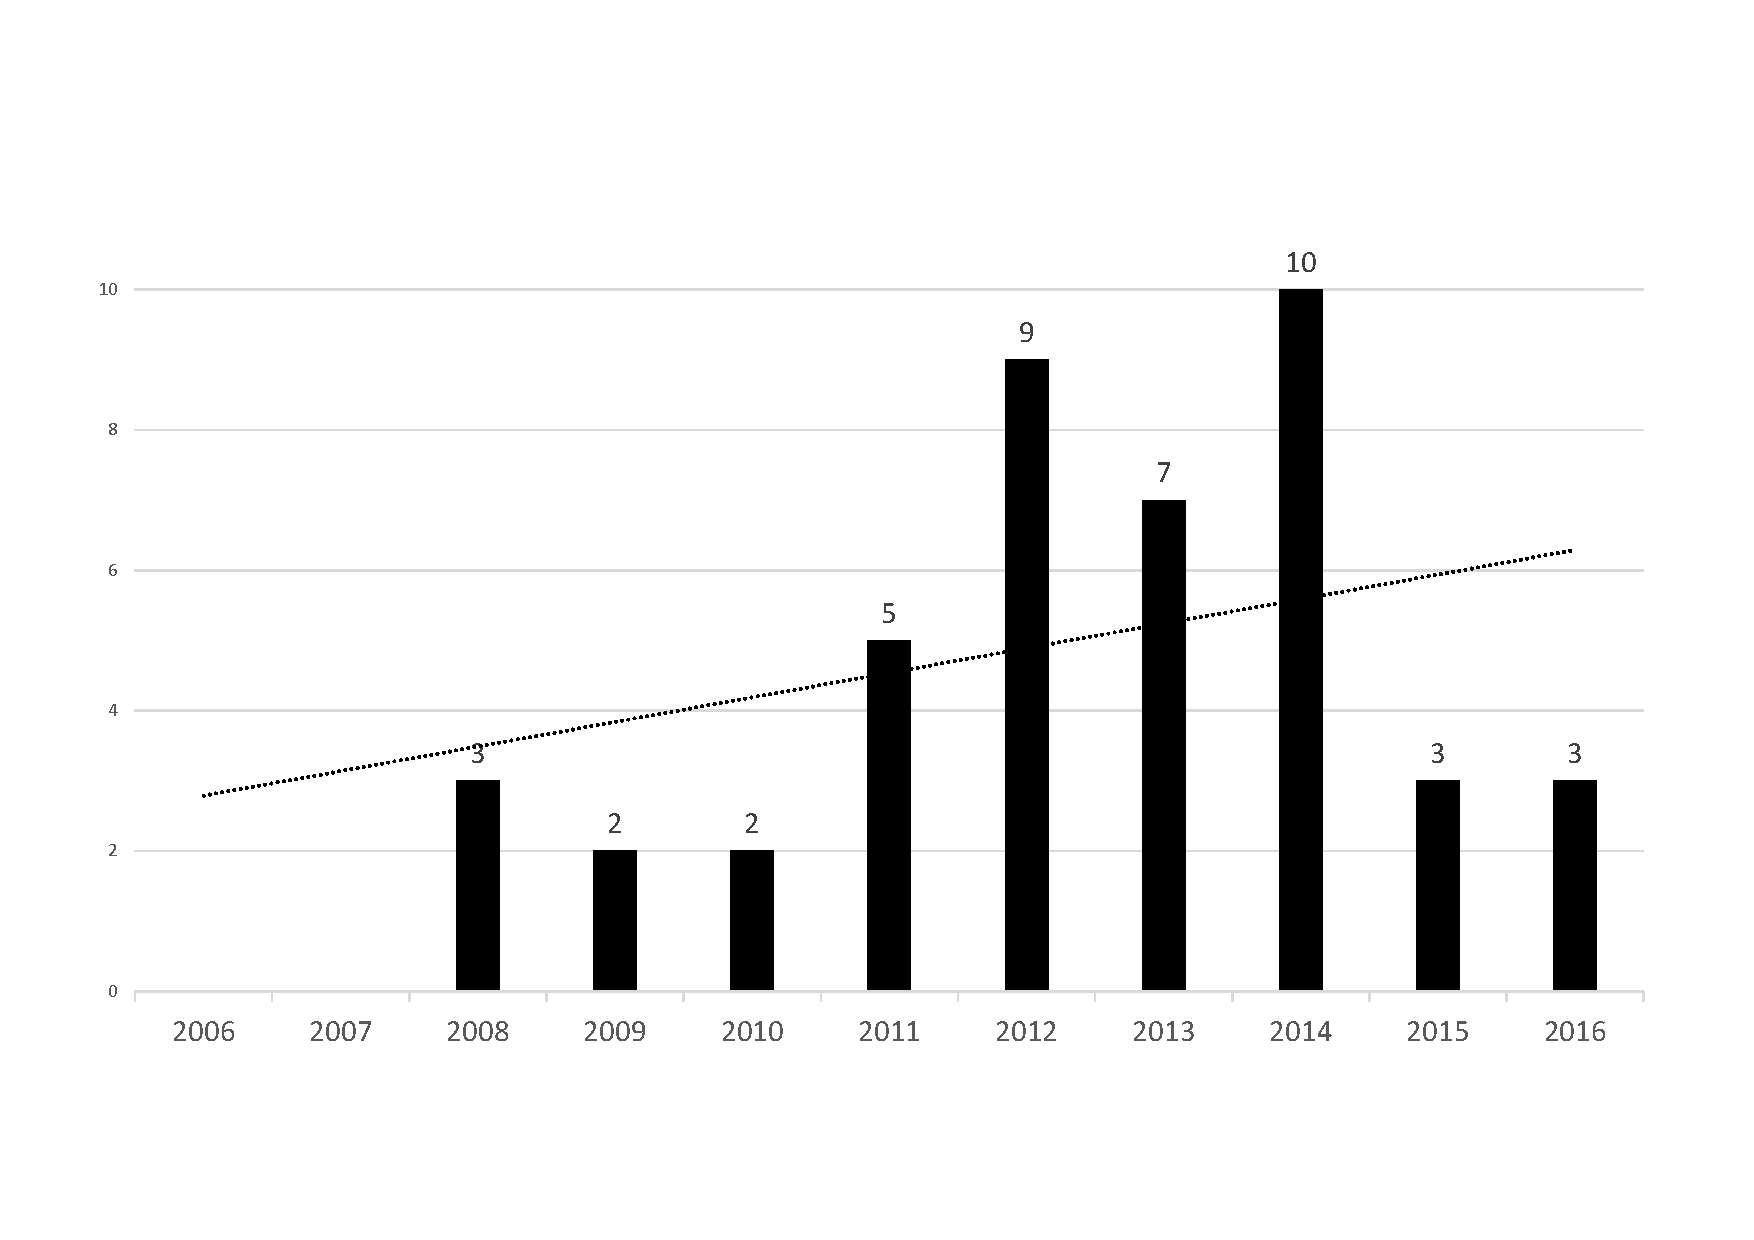
\includegraphics[scale=0.90]{quantidadeano.png}
	\label{fig:qtdano}
\end{figure}
\newpage
\section{Extração de Dados}

\subsection{Trabalhos Selecionados}

Para a extração dos dados, foram considerados 44 trabalhos restantes da 5° lista. Os atributos extraídos são os que estão contidos nas Seção \ref{sec:estrategia}. Os trabalhos utilizados para a extração se encontram na \ref{table:listaextra}

\begin{table}[]
	\centering
	\caption{Trabalhos selecionados para leitura e extração de dados}
	\label{table:listaextra}
	\resizebox{\textwidth}{!}{%
		\begin{tabular}{|c|l|l|c|c|c|c|}
			\hline
			\textbf{ID} & \multicolumn{1}{c|}{\textbf{Título}} & \multicolumn{1}{c|}{\textbf{Autor(res)}} & \textbf{Referência} & \textbf{\begin{tabular}[c]{@{}c@{}}Ano de\\ Publicação\end{tabular}} & \textbf{Fonte} & \textbf{Tipo} \\ \hline
			T1 & \begin{tabular}[c]{@{}l@{}}Delta-Oriented Model-Based SPL\\  Regression Testing\end{tabular} & \begin{tabular}[c]{@{}l@{}}Sascha Lity, Malte Lochau, \\ Ina Schaefer, Ursula Goltz\end{tabular} & \cite{lity2012delta} & 2012 & ACM & Evento \\ \hline
			T2 & \begin{tabular}[c]{@{}l@{}}Industrial Evaluation of Pairwise SPL\\ Testing with MoSo-PoLiTe\end{tabular} & \begin{tabular}[c]{@{}l@{}}Michaela Steffens, Sebastian Oster, \\ Malte Lochau, Thomas Fogdal\end{tabular} & \cite{steffens2012industrial} & 2012 & ACM & Evento \\ \hline
			T3 & \begin{tabular}[c]{@{}l@{}}Model-Based Coverage-Driven Test Suíte\\ Generation for Software Product Lines\end{tabular} & \begin{tabular}[c]{@{}l@{}}Harald Cichos, Sebastian Oster, \\ Malte Lochau, Andy Schurr\end{tabular} & \cite{cichos2011model} & 2011 & ACM & Periódico \\ \hline
			T4 & \begin{tabular}[c]{@{}l@{}}MoSo-PoLiTe - Tool Support for Pairwise\\ and Model-Based Software Product Line\\ Testing\end{tabular} & \begin{tabular}[c]{@{}l@{}}Sebastian Oster, Ivan Zorcic, \\ Florian Markert, Malte Lochau\end{tabular} & \cite{oster2011moso} & 2011 & ACM & Evento \\ \hline
			T5 & MPLM ? MaTeLo Product Line Manager & Hamza Samih, Ralf Bogusch & \cite{samih2014mplm} & 2014 & ACM & Evento \\ \hline
			T6 & \begin{tabular}[c]{@{}l@{}}On the use of test cases in model-based\\ software product line development\end{tabular} & \begin{tabular}[c]{@{}l@{}}Alexander Knapp, Markus Roggenbach, \\ Bernd-Holger Schlingloff\end{tabular} & \cite{knapp2014use} & 2014 & ACM & Evento \\ \hline
			T7 & \begin{tabular}[c]{@{}l@{}}Pairwise Feature-Interaction Testing for\\ SPLs: Potentials and Limitations\end{tabular} & \begin{tabular}[c]{@{}l@{}}Sebastian Oster, Malte Lochau, \\ Marius Zink, Mark Grechanik\end{tabular} & \cite{oster2011pairwise} & 2011 & ACM & Evento \\ \hline
			T8 & \begin{tabular}[c]{@{}l@{}}Deriving Usage Model Variants for Model-\\ based Testing: An Industrial Case Study\end{tabular} & \begin{tabular}[c]{@{}l@{}}Hamza Samih,  Hélène Le Guen, \\ Ralf Bogusch, Mathieu Acher, Benoit Baudry\end{tabular} & \cite{samih2014deriving} & 2014 & IEEE & Evento \\ \hline
			T9 & \begin{tabular}[c]{@{}l@{}}Model-based Software Product Line Testing\\ by Coupling Feature Models with\\ Hierarchical Markov Chain Usage Models\end{tabular} & Ceren Sahin Gebizli, Hasan Sozer & \cite{gebizli2016model} & 2016 & IEEE & Evento \\ \hline
			T10 & \begin{tabular}[c]{@{}l@{}}Model-Based Test Design of Product Lines:\\ Raising Test Design to the Product Line Level\end{tabular} & \begin{tabular}[c]{@{}l@{}}Hartmut Lackner, Martin Thomas, \\ Florian Wartenberg, Stephan Weißleder\end{tabular} & \cite{lackner2014model} & 2014 & IEEE & Periódico \\ \hline
			T11 & \begin{tabular}[c]{@{}l@{}}Requirements-Based Delta-Oriented SPL\\ Testing\end{tabular} & \begin{tabular}[c]{@{}l@{}}Michael Dukaczewski, Ina Schaefer, \\ Remo Lachmann, Malte Lochau\end{tabular} & \cite{dukaczewski2013requirements} & 2013 & IEEE & Evento \\ \hline
			T12 & \begin{tabular}[c]{@{}l@{}}Using Feature Model to Support Model-\\ Based Testing of Product Lines: An \\ Industrial Case Study\end{tabular} & \begin{tabular}[c]{@{}l@{}}Shuai Wang,  Shaukat Ali, \\ Tao Yue, Marius Liaaen\end{tabular} & \cite{wang2013using} & 2013 & IEEE & Periódico \\ \hline
			T13 & \begin{tabular}[c]{@{}l@{}}An automated Model-based Testing\\ Approach in Software Product Lines Using\\ a Variability Language\end{tabular} & \begin{tabular}[c]{@{}l@{}}Boni García,  Rodrigo García-Carmona, \\ Álvaro Navas, Hugo A. Parada-Gélvez, \\ Félix Cuadrado, Juan C. Dueñas\end{tabular} & \cite{garcia2010automated} & 2010 & \begin{tabular}[c]{@{}c@{}}Politécnica Arquivo \\digital UPM\end{tabular} & Evento \\ \hline
			T14 & \begin{tabular}[c]{@{}l@{}}Automated Product Line Methodologies to\\ Support Model-Based Testing\end{tabular} & Shuai Wang,  Shaukat Ali, Arnaud Gotlieb & \cite{wang2013automated} & 2013 & \begin{tabular}[c]{@{}c@{}}CEUR Evento \\ Proceedings\end{tabular} & Evento \\ \hline
			T15 & \begin{tabular}[c]{@{}l@{}}Behavioural Model Based Testing of\\ Software Product Lines\end{tabular} & Xavier Devroey & \cite{devroey2014behavioural} & 2014 & ACM & Evento \\ \hline
			T16 & Feature Model-based Software Product Line Testing & SEBASTIAN OSTER & \cite{oster2012feature} & 2012 & \begin{tabular}[c]{@{}c@{}}TUprints - TU Darmstadt \\ publication service\end{tabular} & Periódico \\ \hline
			T17 & \begin{tabular}[c]{@{}l@{}}Model-based pairwise testing for feature\\ interaction coverage in software product line\\ engineering\end{tabular} & \begin{tabular}[c]{@{}l@{}}Malte Lochau, Sebastian Oster, \\ Ursula Goltz, Andy Schurr\end{tabular} & \cite{lochau2012model} & 2011 & Springer & Periódico \\ \hline
			T18 & \begin{tabular}[c]{@{}l@{}}Model-based Test Generation for Software\\ Product Line\end{tabular} & Xinying Cai, Hongwei Zeng & \cite{cai2013model} & 2013 & IEEE & Evento \\ \hline
			T19 & \begin{tabular}[c]{@{}l@{}}Model-Based Testing for Software Product\\ Lines\end{tabular} & Erika Mir Olimpiew & \cite{olimpiew2008model} & 2008 & Springer & Evento \\ \hline
			T20 & \begin{tabular}[c]{@{}l@{}}PLETS - A PRODUCT LINE OF MODEL-\\ BASED TESTING TOOLS\end{tabular} & ELDER DE MACEDO RODRIGUES & \cite{rodrigues2013plets} & 2013 & PUC-RS & Evento \\ \hline
			T21 & \begin{tabular}[c]{@{}l@{}}Top-Down and Bottom-Up Approach for\\ Model-Based Testing of Product Lines\end{tabular} & Stephan Weißleder, Hartmut Lackner & \cite{weissleder2013top} & 2013 & EPTCS & Evento \\ \hline
			T22 & \begin{tabular}[c]{@{}l@{}}A Product Line Modeling and Configuration\\  Methodology to Support Model-Based \\ Testing: An Industrial Case Study\end{tabular} & \begin{tabular}[c]{@{}l@{}}Shaukat Ali, Tao Yue, Lionel Briand, \\ Suneth Walawege\end{tabular} & \cite{ali2012product} & 2012 & Springer & Periódico \\ \hline
			T23 & \begin{tabular}[c]{@{}l@{}}Coverage Criteria for Behavioural Testing\\  of Software Product Lines\end{tabular} & \begin{tabular}[c]{@{}l@{}}Xavier Devroey, Gilles Perrouin, \\ Axel Legay, Maxime Cordy, \\ Pierre-Yves Schobbens, Patrick Heymans\end{tabular} & \cite{devroey2014coverage} & 2014 & Springer & Evento \\ \hline
			T24 & \begin{tabular}[c]{@{}l@{}}A Model Based Testing Approach for\\  Model-Driven Development and \\ Software Product Lines\end{tabular} & \begin{tabular}[c]{@{}l@{}}Beatriz Pérez Lamancha,  Macario Polo Usaola, \\ Mario Piattini Velthius\end{tabular} & \cite{lamancha2010model} & 2010 & Springer & Evento \\ \hline
			T25 & \begin{tabular}[c]{@{}l@{}}A Vision for Behavioural Model-Driven\\  Validation of Software Product Lines\end{tabular} & \begin{tabular}[c]{@{}l@{}}Xavier Devroey, Maxime Cordy,  Gilles Perrouin, \\ Eun-Young Kang, Pierre-Yves Schobbens, Patrick Heymans,\\  Axel Legay,  Benoit Baudry\end{tabular} & \cite{devroey2012vision} & 2012 & Springer & Evento \\ \hline
			T26 & \begin{tabular}[c]{@{}l@{}}Abstract Test Case Generation for\\  Behavioural Testing of Software Product Lines\end{tabular} & \begin{tabular}[c]{@{}l@{}}Xavier Devroey, Gilles Perrouin, \\ Pierre-Yves Schobbens\end{tabular} & \cite{devroey2014abstract} & 2014 & ACM & Evento \\ \hline
			T27 & \begin{tabular}[c]{@{}l@{}}Applying Incremental Model Slicing to\\  Product-Line Regression Testing\end{tabular} & \begin{tabular}[c]{@{}l@{}}Sascha Lity, Thomas Morbach,  \\ Thomas Th¨ um, Ina Schaefer\end{tabular} & \cite{lity2016applying} & 2016 & Springer & Periódico \\ \hline
			T28 & \begin{tabular}[c]{@{}l@{}}Automated Testing of Software-as-\\ a-Service Configurations using a\\  Variability Language\end{tabular} & Sachin Patel, Vipul Shah & \cite{patel2015automated} & 2015 & ACM & Evento \\ \hline
			T29 & Delta-Oriented FSM-Based Testing & \begin{tabular}[c]{@{}l@{}}Mahsa Varshosaz,  Harsh Beohar,  \\ Mohammad Reza Mousavi\end{tabular} & \cite{varshosaz2015delta} & 2015 & Springer & Evento \\ \hline
			T30 & \begin{tabular}[c]{@{}l@{}}Incremental Model-Based Testing of \\ Delta-oriented Software Product Lines\end{tabular} & \begin{tabular}[c]{@{}l@{}}Malte Lochau, Ina Schaefer, \\ Jochen Kamischke, Sascha Lity\end{tabular} & \cite{lochau2012incremental} & 2012 & Springer & Periódico \\ \hline
			T31 & Model Based Testing in Software Product Lines & \begin{tabular}[c]{@{}l@{}}Pedro Reales, Macario Polo, \\ Danilo Caivano\end{tabular} & \cite{reales2011model} & 2011 & Springer & Evento \\ \hline
			T32 & Model-Based Testing & \begin{tabular}[c]{@{}l@{}}Malte Lochau, Sven Peldszus, \\ Matthias Kowal,  Ina Schaefer\end{tabular} & \cite{lochau2012model} & 2014 & Springer & Evento \\ \hline
			T33 & \begin{tabular}[c]{@{}l@{}}Parameterized Preorder Relations for\\  Model-Based Testing of Software Product Lines\end{tabular} & Malte Lochau, Jochen Kamischke & \cite{lochau2012parameterized} & 2012 & Springer & Evento \\ \hline
			T34 & \begin{tabular}[c]{@{}l@{}}Poster: VIBeS, Transition System\\  Mutation Made Easy,\end{tabular} & \begin{tabular}[c]{@{}l@{}}Xavier Devroey, Gilles Perrouin, \\ Pierre-Yves Schobbens, Patrick Heymans\end{tabular} & \cite{devroey2015vibes} & 2015 & IEEE & Evento \\ \hline
			T35 & Spinal Test Suites for Software Product Lines & Harsh Beohar, Mohammad Reza Mousavi & \cite{beohar2014spinal} & 2014 & EPTCS & Evento \\ \hline
			T36 & \begin{tabular}[c]{@{}l@{}}Automated model-based testing using the\\  UML testing profile and QVT\end{tabular} & \begin{tabular}[c]{@{}l@{}}Beatriz Pérez Lamancha, Pedro Reales Mateo, \\ IgnacioRodríguez de Guzmán, \\ Macario Polo Usaola, Mario Piattini Velthius\end{tabular} & \cite{lamancha2009automated} & 2009 & ACM & Evento \\ \hline
			T37 & \begin{tabular}[c]{@{}l@{}}Relating Variability Modeling and Model-\\ Based Testing for Software Product Lines\\  Testing\end{tabular} & Hamza Samih & \cite{samih2012relating} & 2012 & ICTSS & Evento \\ \hline
			T38 & \begin{tabular}[c]{@{}l@{}}An Evaluation of Model-Based Testing in\\  Embedded Applications\end{tabular} & Stephan Weißleder, Holger Schlingloff & \cite{weissleder2014evaluation} & 2014 & IEEE & Evento \\ \hline
			T39 & \begin{tabular}[c]{@{}l@{}}Assessing Software Product Line Testing\\  Via Model-Based Mutation An \\ Application to Similarity Testing\end{tabular} & \begin{tabular}[c]{@{}l@{}}Christopher Henard, Mike Papadakis, \\ Gilles Perrouin, Jacques Klein, Yves Le Traon\end{tabular} & \cite{henard2013assessing} & 2013 & IEEE & Evento \\ \hline
			T40 & \begin{tabular}[c]{@{}l@{}}Automated and Scalable T-wise Test\\  Case Generation Strategies for \\ Software Product Lines\end{tabular} & Gilles Perrouin, Sagar Sen, Jacques Klein, Benoit Baudry, Yves le Traon Lassy & \cite{perrouin2010automated} & 2010 & IEEE & Evento \\ \hline
			T41 & \begin{tabular}[c]{@{}l@{}}Model-based Testing of System\\  Requirements using UML Use Case Models\end{tabular} & Bill Hasling, Helmut Goetz, Klaus Beetz & \cite{hasling2008model} & 2008 & IEEE & Evento \\ \hline
			T42 & \begin{tabular}[c]{@{}l@{}}Successive refinement of models for\\  model-based testing to increase \\ system test effectiveness\end{tabular} & Ceren Sahin Gebizli, Hasan Sozer, Ali Ozer Ercan & \cite{gebizli2016successive} & 2016 & IEEE & Evento \\ \hline
			T43 & \begin{tabular}[c]{@{}l@{}}A Software Product Line for\\  Model-Based Testing Tools\end{tabular} & \begin{tabular}[c]{@{}l@{}}Elder M. Rodrigues, Avelino F. Zorzo, Itana M. Gimenez, \\ Elisa Y. Nakagawa, Flavio M. Oliveira, José C. Maldonado\end{tabular} & \cite{rodrigues2012software} & 2012 & PUC-RS & Outro \\ \hline
			T44 & \begin{tabular}[c]{@{}l@{}}Reusing State Machines for\\  Automatic Test Generation \\ in Product Lines\end{tabular} & Stephan Weißleder, Dehla Sokenou, Bernd-Holger Schlingloff & \cite{weissleder2008reusing} & 2008 & MoTip & Evento \\ \hline
		\end{tabular}%
	}
\end{table}


\subsection{Qualidade dos Trabalhos}
Para garantir a qualidade dos trabalhos, utilizamos a \ref{table:criterios} de critérios apresentada na Seção \ref{sec:estrategia} para auxiliar na classificação. Seguindo a tabela de questionário, aplicamos o critério aos trabalhos remanescentes para poder levantar quais teriam uma maior relação com o propósito desta RSL.

Sendo assim, originou-se a \ref{table:top10} onde encontram-se os 10 trabalhos com maior relevância e grau de importância em conteúdo, pois possuem uma grande quantidade de dados relacionados diretamente com os objetivos da RSL. Isso não significa que os que não estão listados deixam de ser significativos, somente em nível de quantidade de dados direcionados ao tema.


\begin{table}[]
	\centering
	\caption{Trabalhos com alto valor no critério de seleção}
	\label{table:top10}
	\resizebox{\textwidth}{!}{%
		\begin{tabular}{|c|l|l|c|}
			\hline
			\textbf{ID} & \multicolumn{1}{c|}{\textbf{Título}} & \multicolumn{1}{c|}{\textbf{Autores}} & \textbf{\begin{tabular}[c]{@{}c@{}}Ano de\\ Publicação\end{tabular}} \\ \hline
			T7 & \begin{tabular}[c]{@{}l@{}}Pairwise Feature-Interaction Testing for SPLs: \\ Potentials and Limitations\end{tabular} & \begin{tabular}[c]{@{}l@{}}Sebastian Oster, Malte Lochau,\\  Marius Zink, Mark Grechanik\end{tabular} & 2011 \\ \hline
			T16 & Feature Model-based Software Product Line Testing & Sebastian Oster & 2012 \\ \hline
			T19 & Model-Based Testing for Software Product Lines & Erika Mir Olimpiew & 2008 \\ \hline
			T20 & \begin{tabular}[c]{@{}l@{}}PLETS - A PRODUCT LINE OF MODEL-BASED\\ TESTING TOOLS\end{tabular} & Elder de Macedo Rodrigues & 2013 \\ \hline
			T28 & \begin{tabular}[c]{@{}l@{}}Automated Testing of Software-as-a-Service \\ Configurations using a Variability Language\end{tabular} & Sachin Patel, Vipul Shah & 2015 \\ \hline
			T31 & Model Based Testing in Software Product Lines & \begin{tabular}[c]{@{}l@{}}Pedro Reales, Macario Polo, \\ Danilo Caivano\end{tabular} & 2011 \\ \hline
			T32 & Model-Based Testing & \begin{tabular}[c]{@{}l@{}}Malte Lochau, Sven Peldszus, \\ Matthias Kowal,  Ina Schaefer\end{tabular} & 2014 \\ \hline
			T36 & Automated model-based testing using the UML testing profile and QVT & \begin{tabular}[c]{@{}l@{}}Beatriz Pérez Lamancha, Pedro Reales Mateo, \\ IgnacioRodríguez de Guzmán, Macario Polo Usaola, \\ Mario Piattini Velthius\end{tabular} & 2009 \\ \hline
			T37 & \begin{tabular}[c]{@{}l@{}}Relating Variability Modeling and Model-Based \\ Testing for Software Product Lines Testing\end{tabular} & Hamza Samih & 2012 \\ \hline
			T44 & \begin{tabular}[c]{@{}l@{}}Reusing State Machines for Automatic \\ Test Generation in Product Lines\end{tabular} & \begin{tabular}[c]{@{}l@{}}Stephan Weißleder, Dehla Sokenou, \\ Bernd-Holger Schlingloff\end{tabular} & 2008 \\ \hline
		\end{tabular}%
	}
\end{table}



\subsection{Respostas às Questões de Pesquisa}

Após a leitura dos trabalhos da \ref{table:listaextra} foi possível mapear e extrair informações para contribuir com as respostas para as questões de pesquisa desta RSL.

\subsubsection{QP1: Em quais domínios TBM tem sido aplicado em LPS?} Com relação a primeira pergunta de pesquisa, foram identificados sete domínios distintos, conforme a \ref{table:qpp1}.

O domínio software é o que contém maior incidência com 24 trabalhos, seguido do automotivo com nove, que crescentemente utiliza softwares embarcados em seus produtos.

\subsubsection{Aeroespacial}
MPLM é uma das poucas ferramentas que concentram o maior esforço na questão de solução de variabilidade na geração de casos de teste, \cite{samih2014mplm} em seu trabalho apresentam a ferramenta Matelo, em conjunto com outras ferramentas permite derivar a variante do modelo de um conjunto desejado e assim gerar casos de teste para um projeto experimental na Airbus \textit{defence \& Space}. TBM auxilia no no reaproveitamento para a geração dos casos de teste, o outro trabalho que atua no mesmo domínio é uma extensão deste citado.

\subsubsection{Automotivo}
\cite{lity2012delta} Apresenta uma abordagem delta, que trabalha com elementos transversais de um elemento denominado G, com um conjunto principal e onde os casos de testes estão definidos com cobertura satisfatória. Os artefato de teste são evoluídos de forma incremental, conforme o surgimento de novas variantes do produto. Consideramos que o fator regressão, e adaptabilidade dos artefatos de teste podem conter uma contribuição significativa por serem trabalhados em uma LPS, embora ele não tenha foco em TBM. A utilização de software embarcados nos produtos automotivos cresce exponencialmente, nesse caso levamos em consideração a variação de modelos ofertados, TBM vem auxiliando na geração dos testes destes produtos que sofrem variação, onde existe um núcleo central, e cada variação pode ou não conter uma especificidade única dos demais.

\subsubsection{Eletrônico}
Seguindo este conceito \cite{steffens2012industrial} utiliza de modelos para a geração de subgrupos ou casos de testes a partir destes modelos, aborda a questão de \textit{feature iteractio} com a cobertura de teste e gerencia as variabilidades como itens transversais. MoSo-PoLiTe, ferramenta proposta fazer a derivação dos produtos a partir do modelo principal utilizando de teste combinatório automatizado. TBM atua na geração de casos de teste para subgrupos de produtos, além de buscar garantir uma maior cobertura de erros de funcionalidade, por se tratar de um domínio eletrônico, a garantia da qualidade deve ser com uma margem significativamente maior.

\subsubsection{Manufatura}

\cite{knapp2014use} apresenta um procedimento associado a um conjunto de ferramentas para atribuir o resultado de um caso de teste a um membro arbitrário de uma LPS, usando modelos de variabilidade com base em UML e CVL, utiliza-se do modelo para a criação de máquinas de estado que em seguida são convertidas em diagrama de classe.

\subsubsection{Medicina}
\cite{hasling2008model} realiza a conversão dos modelos em diagramas de atividade e caso de uso, após essa conversão é trabalhado a criação de casos de teste, onde as variantes dos modelos podem ser considerados como variáveis. Por usar TBM, ele não menciona se a variabilidade é tratada, simplesmente utiliza para a criação de casos de teste a partir de diagramas de atividade.

\subsubsection{Software}

Software é um dos domínios mais relatados, a princípio por estar ligado diretamente ao tema da pesquisa, embora os demais domínios também utilizem TBM no processo de desenvolvimento de algum produto de software específico para aquele determinado domínio.

\cite{olimpiew2008model} também proporciona muito dados e informações sobre o TBM em LPS, embora o foco seja em diagramas de atividades customizadas, mas com um foco na reutilização do teste em produtos variantes da LPS. A abordagem proposta CADeT, transforma os casos de uso em diagramas de atividades e que por sua vez são transformados em casos de teste. As especificações de teste são rastreadas a partir do diagrama de atividade e do caso de uso.

A grande maioria dos estudos relatam a criação de alguma abordagem ou ferramenta em TBM para auxílio no desenvolvimento da LPS, no entanto, muitos não deixam bem claro alguns detalhes sobre o propósito principal da utilização de TBM sem seus trabalho. 

\subsubsection{Telecomunicação}
TBM atua no auxilio da derivação de casos de teste a partir de máquinas de estado, a atuação nesse domínio se deve a utilização de meios embarcados nos dispositivos de comunicação. Em determinado momento é possível interpretar que o trabalho referente a este domínio seria manufatura, porém ele tem uma área de atuação bem definida que seria a divisão de pesquisa de uma grande empresa de telecomunicações.

Ainda sobre a utilização de ferramentas \cite{wang2013automated} retrata a utilização de um processo automatizado de seleção de teste de forma minima e sistematizada. Processos automatizados contribuem com algoritmos de seleção, por mais que seja em uma manufatura ele ajuda a criar uma visão sistêmica de seleção de variabilidades. 

\begin{table}[]
	\centering
	\caption{Domínios de aplicação de TBM em LPS}
	\label{table:qpp1}
	\begin{tabular}{|l|l|}
		\hline
		\textbf{Domínio} & \textbf{Referência}                                                                                                                                                  \\ \hline
		Aeroespacial     & T5, T8                                                                                                                                                          \\ \hline
		Automotivo       & T1, T3, T4, T7, T10, T11, T16, T17, T30                                                                                                                              \\ \hline
		Eletrônico       & T2, T9, T42, T44                                                                                                                                                     \\ \hline
		Manufatura       & T6                                                                                                                                                                   \\ \hline
		Medicina         & T41                                                                                                                                                                  \\ \hline
		Software         & \begin{tabular}[c]{@{}l@{}}T13, T15, T18, T19, T20, T21, T23, T24, T25, T26, T27, T28,\\ T29, T31, T32, T33, T34, T35, T36, T37, T38, T39, T40, T43\end{tabular} \\ \hline
		Telecomunicação  & T12, T14, T22                                                                                                                                                        \\ \hline
	\end{tabular}
\end{table}

\subsubsection{QP2: Quais abordagens têm sido utilizadas no TBM de LPS?} Nesse ponto, todos os trabalhos da \ref{table:listaextra} utilizam a abordagem Off-line, que é o teste em tempo de modelagem.

Ainda sobre o contexto da QP2, foram considerados três itens relevantes, técnica de teste utilizada (\ref{table:tecnica}), nível de teste (\ref{table:qpp2}), e automatização de teste utilizada (\ref{table:qpp22}). 


\begin{table}[]
	\centering
	\caption{Níveis de teste aplicado aos trabalhos}
	\label{table:qpp2}
	\begin{tabular}{|l|l|}
		\hline
		\textbf{Nível de teste aplicado} & \textbf{Referência}                                                                                                    \\ \hline
		Desempenho                         & T20                                                                                                                    \\ \hline
		Estrutura                          & T20                                                                                                                    \\ \hline
		Funcionalidade                     & T9, T10, T22, T24, T28, T31, T6                                                                                        \\ \hline
		Integração                         & \begin{tabular}[c]{@{}l@{}}T3, T7, T8, T16, T19, T21, T23, T29, T37, T5, T11,\\ T13, T14,T15, T17, T18\end{tabular} \\ \hline
		Regressão                          & \begin{tabular}[c]{@{}l@{}}T11, T13, T14, T15, T17, T18, T1, T27, T30,\end{tabular}                                 \\ \hline
		Sistema                            & \begin{tabular}[c]{@{}l@{}}T25, T26, T33, T34, T35, T36, T38, T39, T40, T41,\\ T42, T43, T44\end{tabular}        \\ \hline
		Combinatório                       & T4                                                                                                                     \\ \hline
		Unidade                            & T2                                                                                                                     \\ \hline
		Não informado                       & T12, T32                                                                                                               \\ \hline
	\end{tabular}
\end{table}

\begin{table}[]
	\centering
	\caption{Automatização de teste utilizada nos trabalhos}
	\label{table:qpp22}
	\begin{tabular}{|l|l|}
		\hline
		\textbf{Abordagem de teste aplicada} & \textbf{Referência}                                                                                                                                                       \\ \hline
		Automatizada                         & \begin{tabular}[c]{@{}l@{}}T10, T11, T13, T14, T15, T16, T17, T18, T2,\\ T20, T22, T23, T24, T26, T27, T28, T3, T31,\\ T4, T40, T41, T5, T6, T7, T8, T9, T12\end{tabular} \\ \hline
		Semi Automatizada                    & \begin{tabular}[c]{@{}l@{}}T19,T21,T25,T29,T30,T34,T36,T37,T38,T39,\\ T42,T43,T44\end{tabular}                                                                        \\ \hline
		Manual                               & T1, T33, T35                                                                                                                                                              \\ \hline
		Não informado                         & T32                                                                                                                                                                       \\ \hline
	\end{tabular}
\end{table}

Sobre as técnicas utilizadas classificamos como caixa-preta quando não temos acesso ao código somente aos dados que entram e o resultado que deverá sair, já no caixa-branca temos acesso ao código fonte. Os trabalhos estão relacionados conforme a \ref{table:tecnica}.

\begin{table}[]
	\centering
	\caption{Relação de técnicas utilizadas}
	\label{table:tecnica}
	\begin{tabular}{|l|l|}
		\hline
		\textbf{Técnica de Teste} & \textbf{Referência}                                                                                                                                                                                                                                   \\ \hline
		Caixa Preta               & \begin{tabular}[c]{@{}l@{}}T2, T3, T7, T8, T9, T10, T11, T12, T13, T14, T15, T16,\\ T17, T18, T19, T21, T22, T23, T24, T25, T26, T27, T28,\\ T29, T30, T31, T32, T33, T34, T35, T36, T37, T38, T39,\\ T40, T41, T42, T43, T44\end{tabular} \\ \hline
		Caixa Branca              & T1, T4, T20                                                                                                                                                                                                                                           \\ \hline
		Não Informado             & T5, T6                                                                                                                                                                                                                                               \\ \hline
	\end{tabular}
\end{table}

Embora a maior parte dos trabalhos mencione que utiliza uma abordagem automatizada \ref{table:qpp22}, nos trabalhos não se é apresentado como isso é feito, talvez ainda por ser um conceito, ou ainda a falta da implementação da abordagem.




\subsubsection{QP3: Qual o tipo de problema em LPS que TBM tem solucionado?}
Em grande parte TBM está auxiliando na conversão do modelo em artefatos que auxiliem na identificação de possíveis problemas ou erros de interpretação. Representação do comportamento desejado, gerando a partir do caso de teste é algo que torna a cobertura dos erros satisfatória, embora a evolução das técnicas utilizadas durante o processo devem ser aprimoradas. Os modelos servem para serem convertidos, modelados, ou extraídos. Exemplo de comportamento do software.

\subsubsection{QP4: Como variabilidade é tratada no TBM de LPS?}
Na \ref{fig:variabilidade} podemos constatar que a grande maioria dos trabalhos aborda alguma forma gerenciamento de variabilidades, isso demonstra que assim como é crescente o interesse pelo tema, também existe a preocupação com a qualidade, e geral com as variações dos produtos. Na \ref{table:variabilidade} podemos observar quais trabalhos utilizam o gerenciamento de variabilidade durante o processo.

\begin{figure}[htb]
	\centering
	\caption{Proporção dos trabalhos que fazem uso de gerenciamento de variabilidade}
	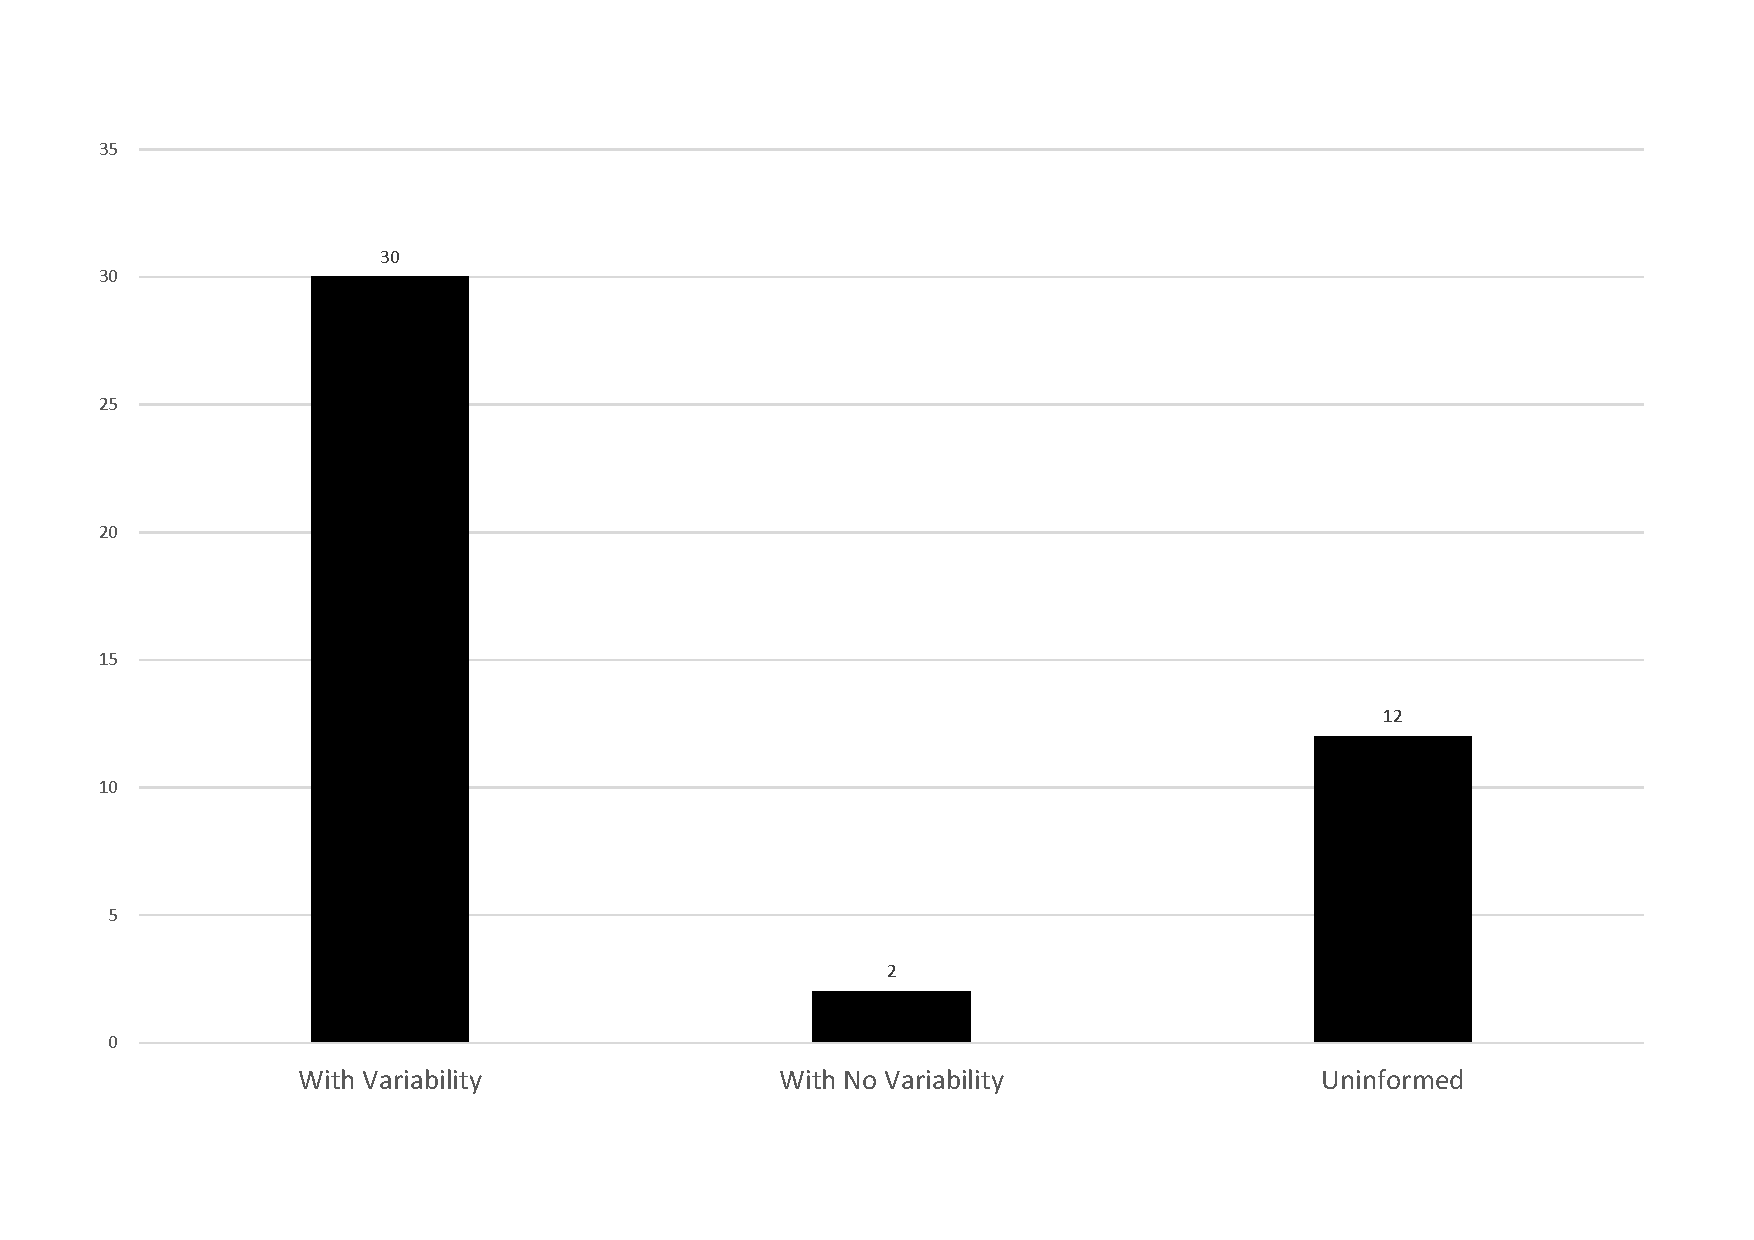
\includegraphics[scale=0.70]{variabilidade.png}
	\label{fig:variabilidade}
\end{figure}

\begin{table}[]
	\centering
	\caption{Trabalhos que consideram gerenciamento de variabilidade durante o processo de teste}
	\label{table:variabilidade}
	\begin{tabular}{|l|l|}
		\hline
		\textbf{\begin{tabular}[c]{@{}l@{}}Gerenciamento de \\ Variabilidade\end{tabular}} & \textbf{Referência} \\ \hline
		Sim & \begin{tabular}[c]{@{}l@{}}T1, T2, T4, T5, T6, T7, T8, T9, T10, T12, T13, T14, T15,\\ T16, T17, T18, T19, T21, T22, T24, T25, T27, T28, T29, \\ T30, T31, T33, T34, T37, T40\end{tabular} \\ \hline
		Não & T39, T43 \\ \hline
		Não informado & \begin{tabular}[c]{@{}l@{}}T3, T11, T20, T23, T26, T32, T35, T36, T38, T41, T42, T44\end{tabular} \\ \hline
	\end{tabular}
\end{table}


\subsubsection{QP5: Como TBM apoia o teste de requisitos não-funcionais?}
Nenhum dos trabalhos apresentados aqui nesta RSL apresenta ou menciona algum tipo de preocupação com requisitos não-funcionais, embora os produtos alvo de teste estejam em tempo de modelagem, nada impede de na criação do plano de teste incluir os requisitos não-funcionais para serem analisados ou verificados.

O ideal seria que todo plano de teste mesmo que em tempo de modelagem contemplasse partes ou a totalidade dos requisitos não-funcionais. Porém, não foram identificadas nesta RSL evidências ou itens que apoiam o teste de requisitos não-funcionais.

\newpage
\subsubsection{QP6: A geração de casos de testes utiliza artefatos ou ferramentas?}
Quando se tem o modelo e parte-se para a geração de casos de teste, muitos dos trabalhos utilizam a conversão do modelo para um determinado artefato intermediário, embora uma certa minoria realize a criação direta do modelo. Na \ref{table:artefatosutilizados} pode-se constatar quantos trabalhos utilizam um determinado artefato para a criação do caso de teste, assim como quais artefatos estão sendo utilizados.


\begin{table}[]
	\centering
	\caption{Artefatos utilizados durante o processo}
	\label{table:artefatosutilizados}
	\begin{tabular}{|l|l|}
		\hline
		\textbf{Artefato IÇntermediário} & \textbf{Referência} \\ \hline
		Máquina de Estado & \begin{tabular}[c]{@{}l@{}}T1, T6, T7, T10, T11, T12, T13, T14, T15, T17,T21,\\ T22, T23, T27, T29, T30, T34, T38, T44\end{tabular} \\ \hline
		Direto do Modelo & T8, T9, T42 \\ \hline
		\begin{tabular}[c]{@{}l@{}}Modelo de variabilidade\\ Ortogonal OVM\end{tabular} & T8 \\ \hline
		Diagrama de Classe & T6, T12, T14, T31 \\ \hline
		Diagrama de Atividade & T18, T19, T41 \\ \hline
		Caso de Uso & T20, T28, T41, T43 \\ \hline
		Diagrama de Sequência & T24, T31, T36 \\ \hline
		Diagrama de Transição & T7, T15, T25, T26, T33, T35, T37 \\ \hline
		Diagrama de Função & T9, T39, T40, T2, T3, T4, T5, T16 \\ \hline
		Não Informa & T32 \\ \hline
	\end{tabular}
\end{table}

Analisando os trabalhos e quais artefatos foram utilizados, constatou-se que muitos além de fazer a utilização de artefatos gerados a partir dos modelos, criam artefatos intermediários, que auxiliam em tomadas de decisões ou que, pela conversão direta do modelo não ser possível para o artefato desejado, se faz por meio de uma dupla conversão.


Assim como os artefatos intermediários levantamos a seguinte situação, utilização de ferramentas durante o processo, na \ref{table:ferramentas} pode ser analisado quais trabalhos fazem uso de ferramentas em qualquer parte do processo, seja para automatização, como auxilio na análise dos dados, etc.

Dentre as ferramentas citadas nos trabalhos, damos destaques as mais citadas, que foram elas: IBM RATIONAL RHAPSODY, MoSo-PoLiTe, MaTeLo Product Line Manager, SPLOT tool, PURE variantes, CADeT Tools, TRUST tool, Pralíntool, VIBeS, Eclipse, UML2 Tools entre outros.

\begin{table}[]
	\centering
	\caption{Trabalhos que fazem uso de ferramentas durante o processo}
	\label{table:ferramentas}
	\begin{tabular}{|l|l|}
		\hline
		\textbf{\begin{tabular}[c]{@{}l@{}}Faz uso de Ferramentas\\ Durante o Processo\end{tabular}} & \textbf{Referência} \\ \hline
		Sim & \begin{tabular}[c]{@{}l@{}}T1, T2, T4, T5, T6, T7, T8, T9, T10, T12, T13,\\ T14, T16, T17, T19, T22, T28, T30, T31, T34,\\ T36, T37, T38, T40, T41, T42\end{tabular} \\ \hline
		Não Informa & \begin{tabular}[c]{@{}l@{}}T3, T11, T15, T18, T20, T21, T23, T24, T25,\\ T26, T27, T29, T32, T33, T35, T39, T43, T44\end{tabular} \\ \hline
	\end{tabular}
\end{table}

\subsubsection{QP7: Quais tipos de modelos de LPS têm sido considerados no TBM?}
Quanto ao tipo de modelo de LPS considerado dentre os trabalhos analisados, a grande maioria se fez da utilização do \textit{Behavioral-based} que se caracteriza por ser comportamental, talvez o motivo seja pelo fato de os modelos serem ricos em detalhes, facilitando a interpretação ou configuração, mesmo que posteriormente o modelo seja convertido em um artefato, primário ou intermediário. Na \ref{table:cenario} pode ser observado que vários trabalhos utilizam o modelo \textit{Scenario-based models} a relação se deve ao fato de estes trabalhos fazerem a utilização de artefatos intermediários, trabalhando com cenários de utilização ao invés de comportamento direto.

\begin{table}[]
	\centering
	\caption{Modelo de LPS considerado nos trabalhos extraídos}
	\label{table:cenario}
	\begin{tabular}{|l|l|}
		\hline
		\textbf{Modelo de LPS Considerado} & \textbf{Referência} \\ \hline
		\textit{Scenario-based models} & \begin{tabular}[c]{@{}l@{}}T3,T11, T19, T20, T24, T31, T38, T40, T41,\\ T42 T43, T44\end{tabular} \\ \hline
		\textit{Class-oriented} & T6 \\ \hline
		\textit{Behavioral-based} & \begin{tabular}[c]{@{}l@{}}T1, T2, T4, T7, T8, T9, T10, T12, T13, T14,\\ T15, T16, T17, T18, T21, T22, T23, T25,\\ T26, T27, T28, T29, T30, T33, T34,T35, T36,\\ T37, T39\end{tabular} \\ \hline
		Não Informado & T5, T32 \\ \hline
	\end{tabular}
\end{table}


\subsubsection{QP8:\textit{Binding time} afeta a aplicação de TBM em LPS?}
Muitas propriedades de um programa são conhecidas durante o processo de execução ou em tempo de desenvolvimento, para isso denominamos \textit{binding time} ou tempo de resolução, neste caso, resolução da variabilidade:\textit{design-time, compile-time, linking-time, runtime}

Nesta RSL, quase que a totalidade dos trabalhos não deixa explícito o \textit{binding time}. Na \ref{table:binding} apresentamos trabalhos que baseado na interpretação dos autores desta RSL, identificaram em algum momento do texto a utilização do \textit{Design Time} como tempo de resolução de variabilidade.


\begin{table}[]
	\centering
	\caption{Estudos que indiretamente relacionam o \textit{binding time}}
	\label{table:binding}
	\begin{tabular}{|l|l|}
		\hline
		\multicolumn{1}{|c|}{\textbf{\begin{tabular}[c]{@{}c@{}}Momento de solução \\ da Variabilidade \\(Binding Time)\end{tabular}}} & \multicolumn{1}{c|}{\textbf{Referência}} \\ \hline
		Design Time & \begin{tabular}[c]{@{}l@{}}T7, T8, T9, T10, T11, T12, T13,T14, T15, T16, T17, T18,\\ T19, T20, T21, T22, T23, T24, T25, T26, T27, T28, T29,\\ T30, T31, T32, T33, T34, T35, T36, T37, T38, T39, T40,\\ T41, T42, T43, T44\end{tabular} \\ \hline
		Não Informa & T1, T2, T3, T4, T5, T6 \\ \hline
	\end{tabular}
\end{table}


\subsubsection{QP9: Como as técnicas e as atividades de TBM para LPS têm sido avaliadas?}
80\% dos trabalhos apresentados (\ref{fig:validacao} e \ref{table:coletaevidencia}) relatam qual foi o método utilizado para a avaliação das atividades. A minoria de 20\% não deixou claro ou não evidenciou se realizou algum tipo de avaliação.

\begin{figure}[htb]
	\centering
	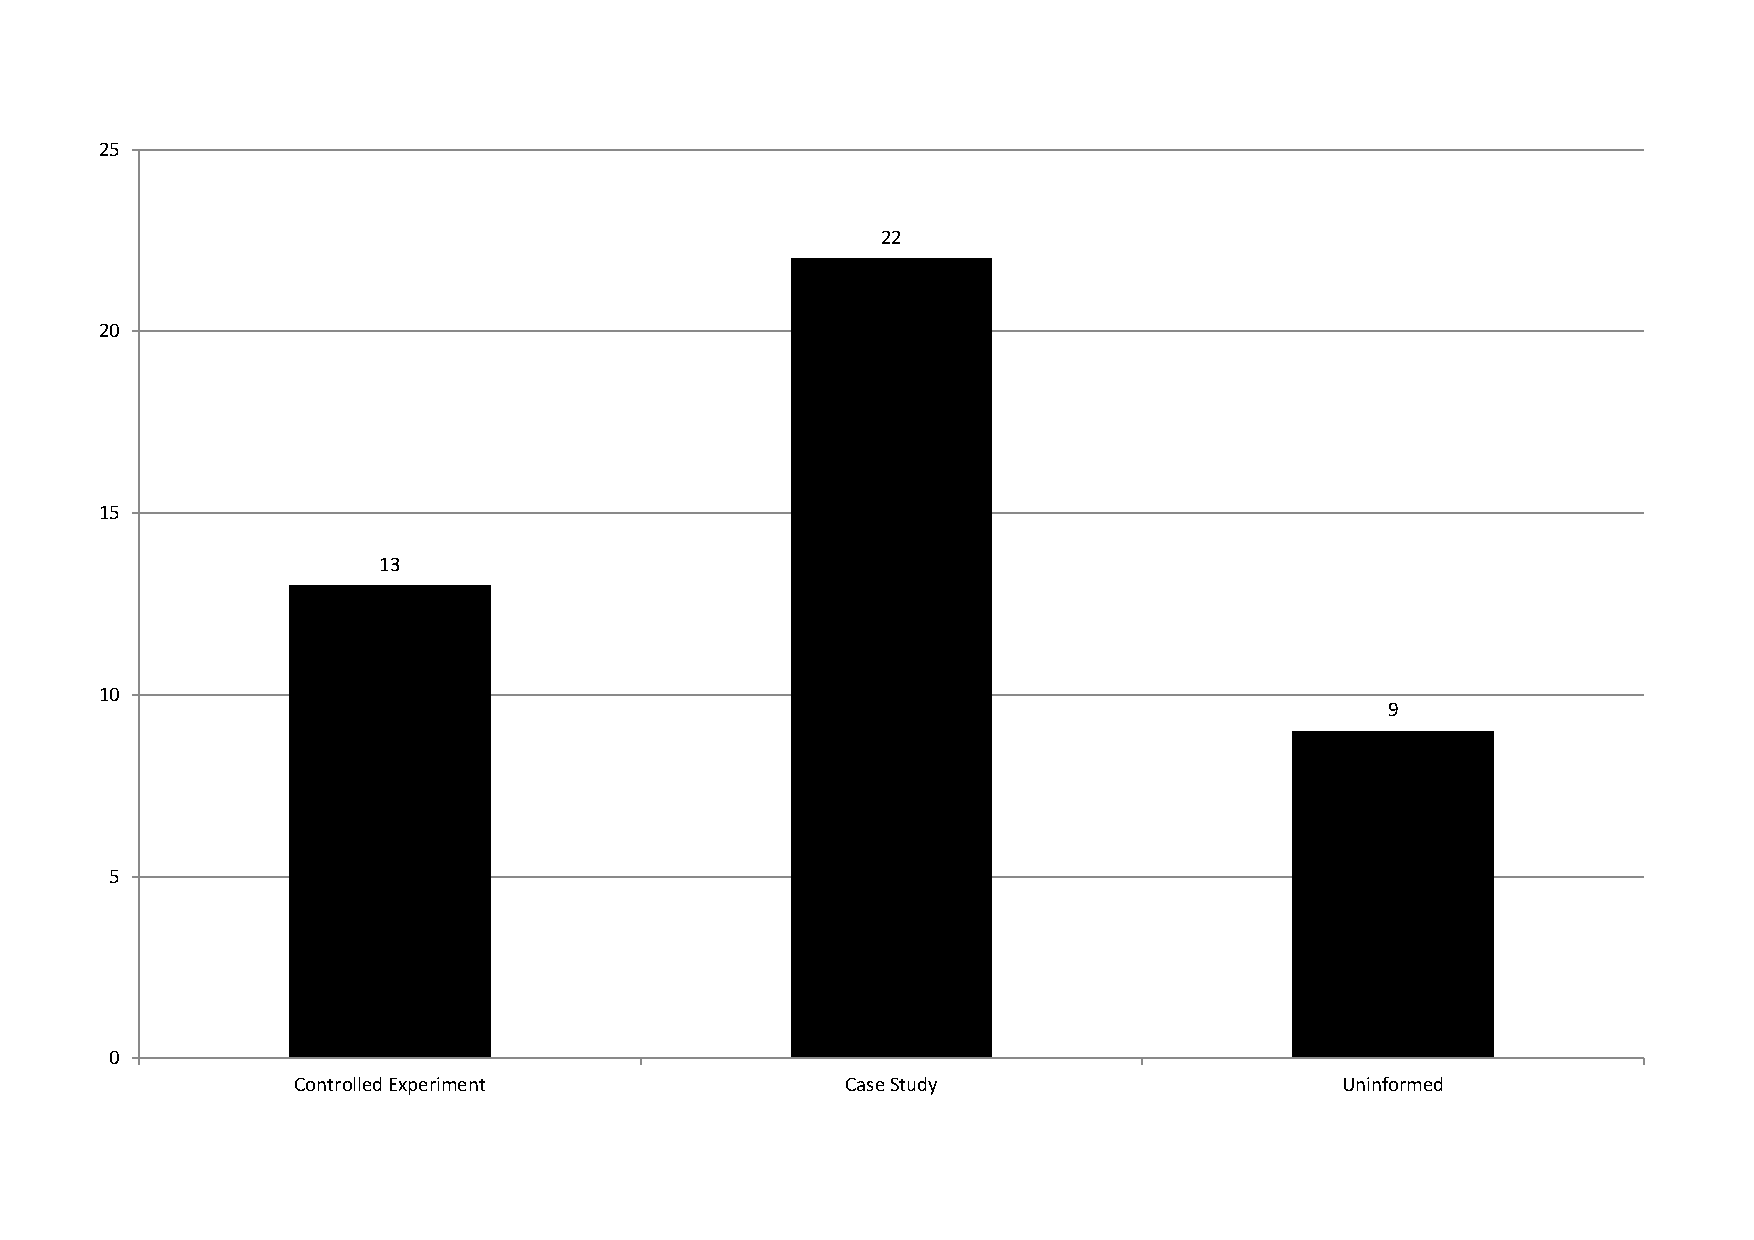
\includegraphics[scale=0.60]{validacao.png}
	\caption{Proporção dos trabalhos que validaram as atividades}
	\label{fig:validacao}
\end{figure}


\begin{table}[]
	\centering
	\caption{Relação de métodos de avaliação utilizados}
	\label{table:coletaevidencia}
	\begin{tabular}{|l|l|}
		\hline
		\textbf{\begin{tabular}[c]{@{}l@{}}Método de Coleta\\ de Evidências\end{tabular}} & \textbf{Referência} \\ \hline
		Experimento Controlado & \begin{tabular}[c]{@{}l@{}}T1, T3, T4, T16, T20, T21, T23, T24, T25, T28, T39, T40,\\ T42\end{tabular} \\ \hline
		Estudo de Caso & \begin{tabular}[c]{@{}l@{}}T2, T6, T7, T8, T9, T10, T11, T12, T13, T14, T15, T17,\\ T19, T22, T26, T27, T29, T30, T33, T38, T43, T44\end{tabular} \\ \hline
		Não evidenciado & T5, T18, T31, T32, T34, T35, T36, T37, T41 \\ \hline
	\end{tabular}
\end{table}

Isso fica evidente quando relatamos os locais de avaliação do trabalho, apresentados na tabela \ref{table:areadevalidacao}. Em análise mais aprofundada, alguns deles por mais que não evidenciem, tendem a ter utilizado estudo de caso como forma de avaliação. 

\begin{table}[]
	\centering
	\caption{Área onde foi avaliado o trabalho}
	\label{table:areadevalidacao}
	\begin{tabular}{|l|l|}
		\hline
		\textbf{\begin{tabular}[c]{@{}l@{}}Área \end{tabular}} & \textbf{Referência} \\ \hline
		Indústria & \begin{tabular}[c]{@{}l@{}}T1, T2, T3, T4, T5, T6, T7, T8, T9, T10, T11, T12, T13,\\ T14, T15, T16, T17, T20, T22, T29, T30, T38, T41, T42,\\ T43, T44\end{tabular} \\ \hline
		Academia & \begin{tabular}[c]{@{}l@{}}T19, T23, T24, T25, T26, T27, T28, T31, T32, T33, T34,\\ T35, T36, T37, T39, T40\end{tabular} \\ \hline
		Não evidenciado & T18, T21 \\ \hline
	\end{tabular}
\end{table}

\newpage
\subsubsection{QP10: É realizado a rastreabilidade em TBM para LPS?}
Ao final da análise dos trabalhos, procuramos encontrar quais foram as principais contribuições apresentadas. Quando falamos em qualidade uma das principais contribuições que esperamos é que sejas contemplados todos ou a maioria do fatores que proporcione qualidade ao produto gerado, além das técnicas, níveis e tipos de testes um ponto que deve ser levado em consideração é o rastreamento das atividades durante o processo.

Ele garante que qualquer alteração que seja realizada possa ser verificada sua origem e alterações, neste quesito podemos conferir na \ref{table:rastreabilidade} quais trabalhos fazem utilização de rastreabilidade, o que gera certa preocupação é que neste ponto, a grande maioria não menciona ou não faz utilização, o que pode gerar inconsistências ou retrabalho. 
\begin{table}[]
	\centering
	\caption{Trabalhos que abordam a utilização de rastreabilidade}
	\label{table:rastreabilidade}
	\begin{tabular}{|l|l|}
		\hline
		\textbf{\begin{tabular}[c]{@{}l@{}}Faz uso de \\ Rastreabilidade\end{tabular}} & \textbf{Referência} \\ \hline
		Sim & T5, T7, T15, T16, T17, T19, T20, T24, T31, T36, T37, T41, \\ \hline
		\begin{tabular}[c]{@{}l@{}}Não faz \\ ou não menciona\end{tabular} & \begin{tabular}[c]{@{}l@{}}T1, T2, T3, T4, T6, T8, T9, T10, T11, T12, T13, T14, T18, T21,\\ T22, T23, T25, T26, T27, T28, T29, T30, T32, T33, T34, T35,\\ T38, T39, T40, T42, T43, T44\end{tabular} \\ \hline
	\end{tabular}
\end{table}

\subsubsection{QP11: Soluções propostas para TBM? }
Além da rastreabilidade, levantamos quais a principais contribuições que os trabalhos apresentam e que pode ser conferido na \ref{table:contribuicao}, podemos constatar que a grande maioria dos trabalhos apresenta como contribuição uma abordagem de utilização ou de processo. Isso demonstra que existe um interesse pela contribuição com novas práticas TBM para LPS.

\begin{table}[]
	\centering
	\caption{Principais contribuições dos trabalhos relacionados}
	\label{table:contribuicao}
	\begin{tabular}{|l|l|}
		\hline
		\textbf{\begin{tabular}[c]{@{}l@{}}Principais Contribuições\\ dos Trabalhos\end{tabular}} & \textbf{Referência} \\ \hline
		Abordagem & \begin{tabular}[c]{@{}l@{}}T1, T5, T6, T7, T8, T9, T10, T11, T13, T14, T15, T16,\\ T17, T18, T20, T21, T22, T23, T24, T27, T28, T29,\\ T30, T31, T35, T36, T37, T38, T39, T41, T42, T43, T44\end{tabular} \\ \hline
		Algoritmo & T3, T25, T26 \\ \hline
		Conjunto de ferramentas & T40 \\ \hline
		Estratégia & T33 \\ \hline
		Extensão de Abordagem & T12 \\ \hline
		Ferramenta & T2, T4, T34 \\ \hline
		Metodologia & T19 \\ \hline
		Tutorial & T32 \\ \hline
	\end{tabular}
\end{table}


\newpage
\section{Discussão Geral}
Esta Seção apresenta um mapeamento de várias questões de pesquisa respondidas nesta RSL com relação aos estudos e as fases do processo de TBM. Três fases consideram, artefato, gerenciamento e verificação e execução da TBM.

\begin{landscape}
	
	\begin{figure}[htb]
		\centering
		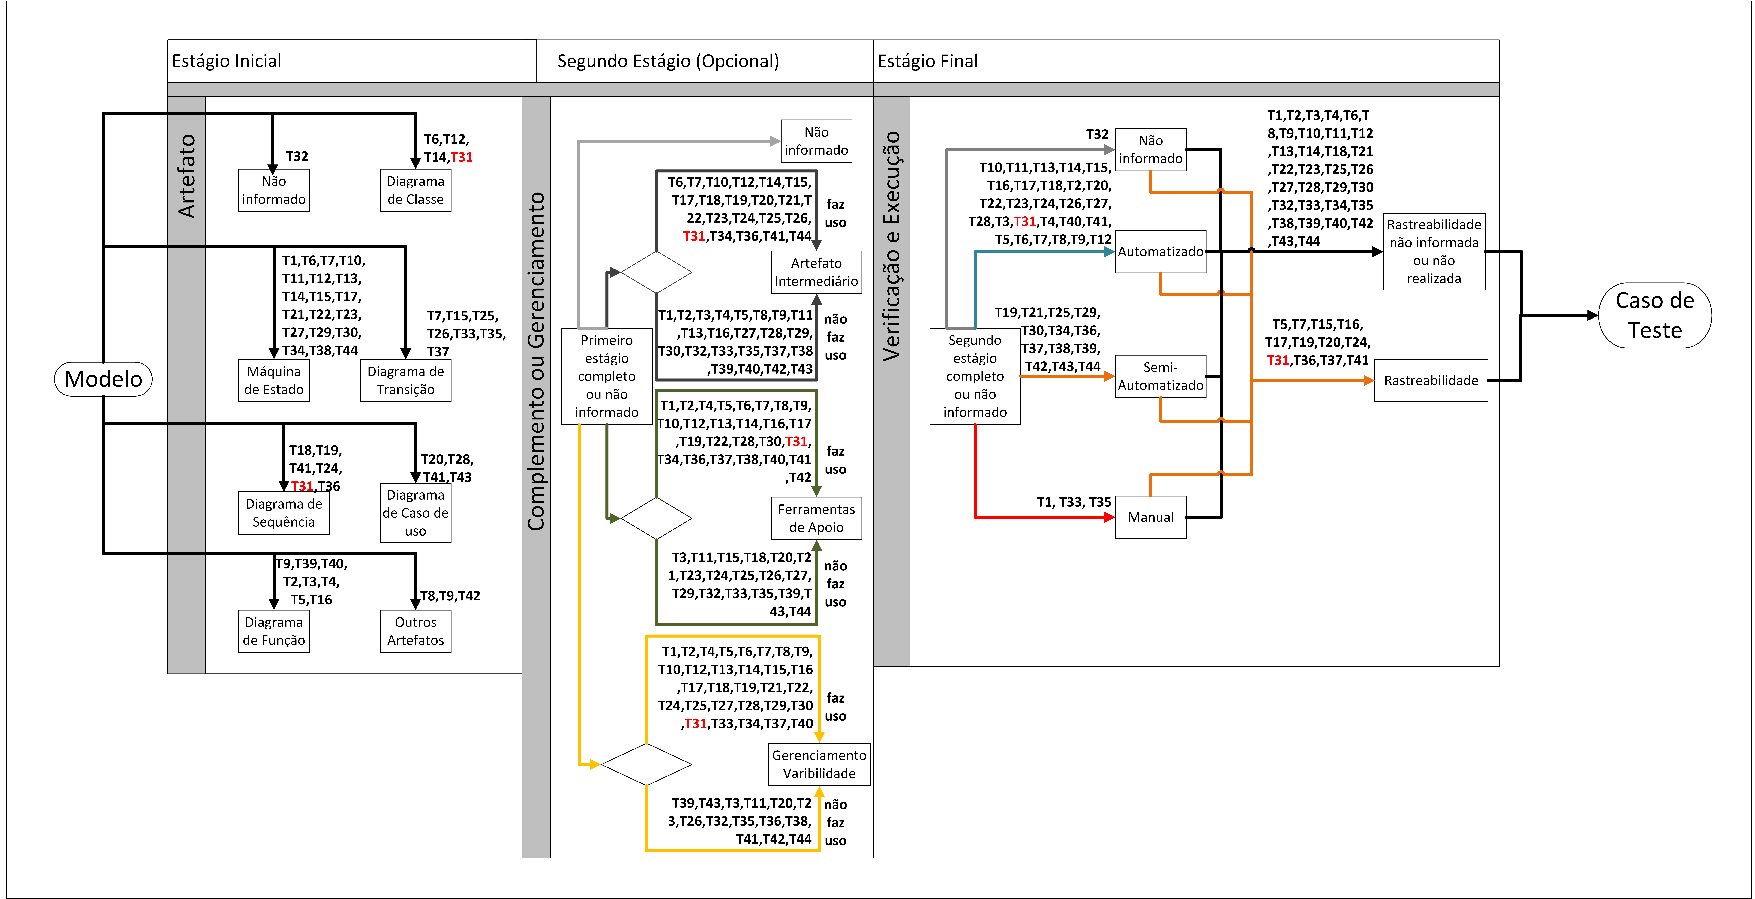
\includegraphics[scale=0.40]{guiaestudo.png}
		\caption{Guia de direcionamento de processo de TBM em LPS}
		\label{fig:guiaestudo1}
	\end{figure}
	
\end{landscape}

Porém, antes temos que explicar alguns conceitos a respeito do guia, para facilitar a busca ou compreensão dele. Após, iremos abordar os principais estudos relacionados e suas contribuições.

A \ref{fig:guiaestudo} apresenta um guia de como os estudos estão divididos de acordo com as fases e atividades de TBM. Para ilustrar o guia serão apresentados dois cenários: o primeiro em que se deseja saber o ciclo completo, a partir de um modelo até a geração de casos de teste, e suas etapas para um determinado trabalho; e o segundo cenário, em que a busca se dá pelo tema e não pelo trabalho, o que permite saber quais trabalhos, por exemplo, fazem uso de ferramentas de apoio, ao TBM.

\subsubsection{Cenário 1 - Percurso por Trabalho}

Digamos que ao selecionar um trabalho da \ref{table:listaextra} a partir de sua ID deseja-se verificar no guia da \ref{fig:guiaestudo} qual caminho ele percorre identificando os seus estágios e as suas atividades. Sendo assim, inicialmente analisarmos o primeiro estágio representado na \ref{fig:estagio1}, que é um excerto da \ref{fig:guiaestudo}.

\begin{figure}[htb]
	\centering
	\includegraphics[scale=0.80]{estagio1.png}
	\caption{Estágio Inicial do processo de TBM em LPS}
	\label{fig:estagio1}
\end{figure}
Pega-se, por exemplo, o trabalho T31. A partir de um modelo, T31 faz uma conversão para o artefato diagrama de sequência, assim podemos considerar o T31. Com o estágio inicial concluído, o segundo estágio (opcional) é então iniciado e T31 considera gerenciamento de variabilidade, apoio de ferramentas, e geração de artefatos intermediários, visto que neste estágio abordamos gerenciamento de variabilidade, uso de ferramentas, geração de artefatos intermediários e caso ele não realize nenhuma dessas atividades automaticamente ele poderia estar na geração de caso de teste.


\begin{figure}[htb]
	\centering
	\includegraphics[scale=0.80]{estagio2.png}
	\caption{Segundo estágio do processo de TBM em LPS}
	\label{fig:estagio2}
\end{figure}

\begin{figure}[htb]
	\centering
	\includegraphics[scale=0.80]{estagio3.png}
	\caption{Estágio final do processo de TBM em LPS}
	\label{fig:estagio3}
\end{figure}

Apresentando o estágio final na \ref{fig:estagio3} pode-se analisar que o trabalho T31 faz uso de processo automatizado e utiliza rastreabilidade durante o processo. Assim, completa-se o percurso do para para o trabalho T31 e assim identificar por quais etapas o trabalho reportou.

\subsubsection{Cenário 2 - Percurso por Tema}
O segundo cenário realiza o percurso por tema da TBM em LPS por assunto. Analisando a \ref{fig:estagio3}, por exemplo, pode-se verificar quais os trabalhos que fazem o uso de rastreabilidade. Portanto, se o interesse do leitor for por trabalhos que fazem o uso de rastreabilidade basta simplesmente remeter-se à essa atividade para se obter a lista de tais trabalhos.



\subsubsection{Estudos Secundários}
Para garantir a qualidade e confiança das informações relatadas neste trabalho, realizamos uma busca por estudos secundários sobre o tema. 
\cite{isa2017model} apresenta uma RSL sobre TBM para LPS, porém, consideramos que por ter deixado de seguir alguns padrões recomendados por \cite{kitchenham2004procedures}, ele apresenta inúmeras ameaças a validade além de não poder ser replicado. 

No estudo ele cita que indica modelos e estratégias utilizados, porém não apresenta dados e nem indicadores de quais estudos levantados apresenta tais itens. A quantidade de trabalhos reportados pela \textit{string} de busca está muito abaixo do reportado por esta RSL, devido a baixa cobertura de palavras chave.

Relata que cobre os problemas que foram resolvidos utilizando TBM, mas apresenta dois ou três tipos que já vem sendo reportados em teste em LPS, não agrega quais soluções estão sendo utilizadas. Além de outros fatores não reportados como, variabilidade, tipos de modelos formais utilizados, uso de ferramentas de apoio, geração de casos de teste entre outros. Por isso achamos necessário a realização deste estudo secundário, devido a grande quantidade de informações não reportadas.

\subsubsection{Trabalhos Relacionados}
Dos 44 trabalhos restantes, procuramos delinear um caminho de informações que ampliassem a visão sobre TBM em LPS com foco em variabilidade, assim, o objetivo desta seção é apresentar os fatos principais de cada trabalho referente ao objetivo da RS.

\cite{lity2012delta} Apresenta uma abordagem delta, que trabalha com elementos transversais de um elemento denominado G, com um conjunto principal e onde os casos de testes estão definidos com cobertura satisfatória. Os artefato de teste são evoluídos de forma incremental, conforme o surgimento de novas variantes do produto. Consideramos que o fator regressão, e adaptabilidade dos artefatos de teste podem conter uma contribuição significativa por serem trabalhados em uma LPS, embora ele não tenha foco em TBM.

Seguindo este conceito \cite{steffens2012industrial} utiliza de modelos para a geração de subgrupos ou casos de testes a partir destes modelos, aborda a questão de \textit{feature iteractio} com a cobertura de teste e gerencia as variabilidades como itens transversais. MoSo-PoLiTe, ferramenta proposta fazer a derivação dos produtos a partir do modelo principal utilizando de teste combinatório automatizado.

\cite{cichos2011model} aborda a questão dos conflitos da engenharia com os padrões ISO 26262 onde exige que cada configuração critica de segurança tenha bem definido os critérios de cobertura, assim ele buscar abordar este dilema apresentando um conjunto de teste com base em algoritmo de geração que usa técnicas de teste baseada em modelos, com isto eles pretendem fazer a geração completa de testes para a LPS. Isso se torna interessante no ponto de vista de que teste exaustivo é inviável, talvez com a implementação de um algoritmo fazendo o trabalho de combinação pode ser que esse viés seja contornado.

\cite{oster2011moso} traz um estudo prévio ao \cite{steffens2012industrial} que apresenta a ferramente MoSo-PoLiTe, voltado para a geração de \textit{scripts} de teste a partir de modelos, se os mesmo princípios apresentados por \cite{steffens2012industrial}, o que agrega é o detalhamento de como o processo automatizado é realizado.

MPLM é uma das poucas ferramentas que concentram o maior esforço na questão de solução de variabilidade na geração de casos de teste, \cite{samih2014mplm} em seu trabalho apresentam a ferramenta Matelo, em conjunto com outras ferramentas permite derivar a variante do modelo de um conjunto desejado e assim gerar casos de teste para cada variante.
Ainda que ele utilize modelos ortogonais, contribui muito para o TBM em LPS principalmente no quesito gerenciamento de variabilidade.

\cite{knapp2014use} apresenta um procedimento associado a um conjunto de ferramentas para atribuir o resultado de um caso de teste a um membro arbitrário de uma LPS usando modelos de variabilidade com base em UML e CVL, soma mais uma visão sobre como realizar o gerenciamento de variabilidades em uma LPS conforme a variação do produto.

Nesta fase podemos observar que a grande maioria dos estudos utilizam-se de artefatos de máquinas de estado, \cite{oster2011pairwise} trabalha com a conversão do modelo em máquina de estado, ele aborda que as características de \textit{feature interaction} são uma base para um modelo de falha, pois são reveladas normalmente durante a execução e troca de informações. 

O critério é cobrir quantas interações entre diferentes recursos possíveis, aumentando assim a probabilidade de encontrar erros, neste caso eles propõem uma abordagem combinatória de recursos para a realização de uma cobertura abrangente, no caso uma maior cobertura de interações de recursos é alcançada em uma fração custo menor. A contribuição para nosso trabalho seria o sistema de mapeamento de \textit{feature} assim como a combinação das interações para análise de cobertura, podemos considerar que ele aborda os principais pontos desta pesquisa, onde ele utiliza ferramentas, faz o gerenciamento das variabilidades, além de prover a rastreabilidade durante o processo.

\cite{samih2014deriving} é um complemento do trabalho de \cite{samih2014mplm} abordagem que adota TBM, ela esta integrada a ferramenta apresentada por \cite{samih2014mplm}.

Pensando em uma abordagem para a reutilização sistemática dos modelos para se testar uma grande família de produtos, \cite{gebizli2016model} se fizeram utilizar da cadeia hierárquica de Markov esses modelos captura todos os possíveis cenários de uso para uma família de sistemas, assim como documentar a variabilidade explicitamente e separadamente com um recurso modelo.

\cite{lackner2014model} buscam a geração de casos de teste no nível da LPS, no caso eles estão atuando em um domínio automotivo, mas podemos extrair algumas técnicas visando a questão de conversão do modelo e a verificação da variação do produto, que não fica atrelado ao item principal.

Quando abordamos variabilidade, um do maiores problemas é a reutilização do mesmo caso de teste quando existe uma variável do produto, seguindo a mesma linha de \cite{lity2012delta}, \cite{dukaczewski2013requirements} aborda a modelagem delta para utilização em LPS menos formal. Eles apresentam dados relacionados ao alto índice de reuso em contraste com o baixo numero de reteste, se os casos não forem totalmente compatíveis.

\cite{wang2013using} aborda que no contexto de TBM em LPS o esforço para desenvolver modelos pode ser significativamente reduzido caso seja utilizado uma metodologia de modelagem e configuração sistemática, para isso apresentam uma metodologia que captura a variabilidade em máquina de estado UML e gera os casos de testes a partir destes artefatos e com a ajuda de uma ferramenta gera os testes executáveis. A contribuição esperada é a forma como os processos podem ser automatizados na geração dos casos de teste.

\cite{garcia2010automated} Apresenta uma abordagem de teste automatizado para LPS, utilizando máquina de estado e modelo de variabilidade, o teste baseado em modelo fornece uma técnica para automação e geração de casos de teste usando modelos UML, trabalho importante contextualizando o método utilizando ferramentas como \textit{JUnit Test Suite} onde é apresentado todo o processo de automatização.

Ainda sobre a utilização de ferramentas \cite{wang2013automated} retrata a utilização de um processo automatizado de seleção de teste de forma minima e sistematizada. Processos automatizados contribuem com algoritmos de seleção, por mais que seja em uma manufatura ele ajuda a criar uma visão sistêmica de seleção de variabilidades. 

Essa visão sistêmica pode ser visualizada também em \cite{devroey2014behavioural} onde utiliza uma linguagem de especificação de variabilidades TVL, e utiliza os modelos para criação de \textit{statecharts} para identificação das variabilidades, a partir deles criar os cenários para testes.

Assim como \cite{oster2012feature} que faz das mesmas atribuições durante o processo, apresenta um trabalho com um conteúdo de \textit{background} muito rico de informações sobre variabilidade e reuso em LPS, além dos principais pontos de teste em LPS. Apresenta também uma proposta de teste combinatório bem extensa, onde não utiliza conversão do modelo para a geração dos casos de teste.

A contribuição do trabalho esta relacionado diretamente a quantidade de dados e informações relacionadas, os principais elementos necessários para a criação de uma visão macro sobre teste, variabilidade, modelos em LPS, além de apresentar uma gama de ferramentas que foram utilizadas durante o processo.

\cite{lochau2012model} faz continuidade do estudo de \cite{oster2011pairwise} adicionando uma definição concisa de dependências de recursos e interações de características do ponto de vista do teste, e discutem os critérios de adequação para a cobertura paralela em SPL, apresentam testes de interação e dão uma generalização ao caso T-wise.

Seguindo a geração de casos de teste a partir da SPL, \cite{cai2013model} trazem uma abordagem baseada em modelo para testar geração de casos de testes para SPLs, onde possa ser reutilizável esses cenários de teste e de domínio que são gerados a partir de diagramas de atividades estendido com pontos de variação e, em seguida, teste dos cenários de acordo com os pontos de variação.

\cite{olimpiew2008model} também proporciona muito dados e informações sobre o TBM em LPS, embora o foco seja em diagramas de atividades customizadas, mas com um foco na reutilização do teste em produtos variantes da LPS. A abordagem proposta CADeT, transforma os casos de uso em diagramas de atividades e que por sua vez são transformados em casos de teste. As especificações de teste são rastreadas a partir do diagrama de atividade e do caso de uso.

A contribuição seria relacionada ao processo de reutilização de caso de teste conforme a mudança de característica do produto, pois segundo a abordagem, pode ser usado para criar especificações de teste reutilizáveis para cobrir todos cenários de casos de uso.

Trabalhando a partir de casos de uso \cite{rodrigues2013plets}, a ferramenta PLETS procura trabalhar uma LPS de ferramentas de teste que tenham suporte a TBM e um ambiente automatizado para apoiar a geração dessas ferramentas. Podemos considerar que as contribuições para o trabalho é o meio modelo do processo de geração de \textit{scripts} de teste, que foi comparado com uma ferramente \textit{Capture and replay} e obteve um desempenho melhor.

Compartilhando um visão \textit{top down} \cite{weissleder2013top} utiliza os modelos em conjunto com a modelagem de recursos e comportamento em uma visão \textit{top down} para a geração de diagramas de estado e comportamento, contribuem para uma visão macro da modelagem como um todo e os processos bem definidos. Algo interessante realizado neste estudo é que modelagem de recursos e design de teste baseado em modelo, essa combinação no entanto, raramente foi o foco da investigação.

Máquinas de estado são também utilizadas por \cite{ali2012product} onde os modelos são convertidos, e através deles é que se faz a verificação de variabilidade.

\cite{devroey2014coverage}Utiliza de uma estrutura matemática para representar o comportamento de uma forma concisa onde os modelos utilizados para a extração de máquinas de estado e a partir dai a geração de casos de teste. Não deixa explicito o gerenciamento de variabilidade, mas ele utiliza do critério de combinação para controlar as possíveis variações de funções existentes.

Já \cite{lamancha2010model} utiliza o modelo de variabilidade Ortogonal OVM, já os modelos são convertidos em modelos de design e a partir deles são gerados os modelos de teste.

\cite{devroey2012vision} realiza a utilização do modelo para a criação de um padrão de QA, composto por 3 etapas, modelagem, \textit{design} e validação. A partir do modelo é gerado o comportamento esperado e assim criado os diagramas de transições entre os estados, assim, a variabilidade é tratada durante a geração dos diagramas de máquinas de estado, quando gerado os casos de testes é verificado sua abrangência de cobertura.

\cite{devroey2014abstract} faz a utilização de algoritmo matemático para a classificação dos modelos conforme critérios pré definidos pelo usuário, assim os modelos serão utilizado para a criação de máquinas de estados e a partir disso realizar a derivação de casos de testes a partir do comportamento destes modelos.Não menciona se faz o gerenciamento de variabilidade, devido a geração de casos de teste ser automatizada por algoritmo, então ele busca gerar todos os casos de testes possíveis baseado no critério de cobertura especificado pelo engenheiro de teste.

Utilizando-se do modelo para verificação do comportamento entre os mesmos quando ocorrido alterações,\cite{lity2016applying} faz uma análise dos casos de testes gerados, para assim a geração de novos casos de testes serem condizentes e para utilização em casos de reteste.
As variabilidades são tratadas através de modelagem orientada a Delta, onde é criado um núcleo comum e as variantes são tratadas como variantes deste núcleo, tem se um núcleo comum e adaptações do mesmo para os demais artefatos.

A Criação de um modelo base para poder obter uma análise de variabilidades, após realizar a geração de scripts de teste conforme a especificação da variabilidade, é o que propõe \cite{patel2015automated}. Tratar as variabilidades a partir de um modelo padrão que é criado para extração de casos de teste.

\cite{varshosaz2015delta} faz a utilização dos modelos para conversão em diagramas de estado finito, já na modelagem delta é trabalhado um modelo núcleo que a partir dele se derivam as funcionalidades, trabalho similar ao de \cite{lity2016applying} e \cite{lochau2012incremental}, embora a variabilidade seja tratada de forma que um núcleo comum é criado e as variações geradas a partir deste núcleo comum é que são tratadas como variabilidade.

\cite{reales2011model},\cite{lochau2012parameterized}, \cite{lamancha2009automated} e \cite{samih2012relating} Trabalham diretamente dos modelos e são exclusivamente utilizados para a geração dos diagramas necessários para a criação dos casos de teste, e no quesito de variabilidade é modelado utilizando notação ortogonal OVM.
Já \cite{weissleder2014evaluation} trabalha a partir do modelo mas não faz uso de OVM.

\cite{lochau2012model}Utiliza o modelo como uma abordagem formal para o teste funcional dinâmico, basear todas as atividades de teste em um modelo de teste formal do comportamento esperado.
Menciona que existe um controle sobre as variabilidades, mas não explica de qual forma isso é feito, relata que existem técnicas de gestão de variabilidades que são trabalhadas em conjunto com a abordagem, mas não menciona quais.

\cite{devroey2015vibes} trabalha com os modelos convertidos em máquinas de estados finito para a verificação das variáveis. Através de um quadro onde é analisado a mutação e apresentado todas as variabilidades existente em um único modelo.

Modelo convertido em sistema de transição é então analisado todas as possíveis variáveis, porém \cite{beohar2014spinal} não menciona se é feito alguma modelagem, só aborda que os testes criados são trabalhados como uma coluna vertebral onde os novos recursos são testados e agregados a esse volume central.

Faz uso para a criação de modelos similares com erros incluídos de forma proposital afim de garantir que a técnica de teste seja eficaz, \cite{henard2013assessing} não aborda o ponto de variabilidade, visa somente a derivação de modelos para os testes.

Os modelos são derivados em submodelos e para em seguida serem utilizados para a geração de casos de testes, e por utilizar uma gama de ferramentas as variabilidades são tratadas na geração dos casos de teste onde os modelos originados em submodelos dos modelos principais segundo \cite{perrouin2010automated}

\cite{hasling2008model} realiza a conversão dos modelos em diagramas de atividade e caso de uso, após essa conversão é trabalhado a criação de casos de teste, onde as variantes dos modelos podem ser considerados como variáveis, mas não relata como e onde esse ponto é tratado durante o processo. De forma similar \cite{gebizli2016successive} trabalha o modelo refinando até se chegar aos processos de transições, mas não menciona se é tratada a variabilidade ou como seria tratado, o foco fica somente nos modelos.

\cite{rodrigues2012software}Utiliza a arquitetura de referência que suporta MBT em LPS, não modela a variabilidade, ficando a cargo de um plugin de terceiro por este trabalho. Ao contrário de \cite{weissleder2008reusing} que apresenta um novo método de utilização do modelo em formato de máquina de estado onde variabilidade é expressada por pré ou pós condições ou valores de atributos de classe correspondente.



\section{Ameaças à Validade}
0As seguintes ameaças à validade deste estudo são discutidas:

\begin{itemize}
	\item Questão de Pesquisa: o objetivo desta RSL foi encontrar estudos publicados que abordam TBM em LPS. De acordo com essa condição, onze questões de pesquisa com abrangência ao objetivo foram definidas para este estudo. assim, outras questões importantes podem ter ficado de fora deste estudo e, portanto, assuntos pertinentes à esta revisão podem não ter sido abordados.
	\item Viés de Publicação: não é possível garantir que todos os estudos primários relacionados com o tema deste estudo secundário foram encontrados. Esse problema pode ocorrer porque os motores de busca não são tão precisos como se deseja para o processamento e execução de consultas de acordo com as palavras-chaves definidas.
	\item O protocolo desta RSL foi revisado por outros pesquisadores, e isso pode diminuir as ameaças a este estudo.	

	
\end{itemize}


\section{Considerações Finais}
Após a análise dos dados extraídos da RSL realizada, foi possível constatar e identificar quais as técnicas de teste TBM utilizadas, e quais utilizam notação UML, os trabalhos que realizam um controle de variabilidade, assim como a rastreabilidade. Também como são gerados os casos de testes, de forma manual ou automatizada.

As contribuições para o TBM em LPS são ricas em detalhes quanto os artefatos utilizados, as técnicas reportadas, utilização de ferramentas e uso do gerenciamento de variabilidades, são os principais dados que esta RSL contribui de maneira geral.

Em resumo, existe um crescente interesse pelo tema, embora não podemos identificar o porque da rastreabilidade e os teste de requisitos não funcionais, não estarem explicitamente apresentados, estudos mais aprofundados sobre essas duas temáticas poderão dizer mais a respeito.

Um dos pontos principais que é o gerenciamento de variabilidade atrelado ao modelo em LPS, foi apresentado por uma maioria significativa, isso demonstra que existe uma crescente consciência relacionado qualidade do produtos variantes originados de um produto principal.


